%% File encoding: UTF-8
%% äöüÄÖÜß  <-- keine deutschen Umlaute hier? UTF-faehigen Editor verwenden!

\documentclass[bachelor,german]{hgbthesis}
% Zulässige Class Options: 
%   Typ der Arbeit: diplom, master (default), bachelor, praktikum 
%   Hauptsprache: german (default), english
%%------------------------------------------------------------

\RequirePackage[utf8]{inputenc}		% remove when using lualatex oder xelatex!

\graphicspath{{images/}}    % name of directory containing the images
\logofile{logo}							% name of logo-PDF in images/ (or use \logofile{} for no logo)
\bibliography{literatur}  	% name of the BibTeX (.bib) file

\usepackage{pdfpages}
\usepackage{listings}
\usepackage{graphicx}
\usepackage{tikz}
\usepackage{pgfplots}
\usepackage{subfig}
\usepackage{minitoc}
\usetikzlibrary{
  arrows.meta, % for Straight Barb arrow tip
  fit, % to fit the group box around the central neurons
  positioning, % for relative positioning of the neurons
}

\tikzset{
  neuron/.style={ % style for each neuron
    circle,draw,thick, % drawn as a thick circle
    inner sep=5pt, % no built-in padding between the text and the circle shape
    minimum size=1.5em, % make each neuron the same size regardless of the text inside
    node distance=1ex and 3em, % spacing between neurons (y and x)
  },
  group/.style={ % style for the groups of neurons
    rectangle,%,draw,thick, % drawn as a thick rectangle
    inner sep=0pt, % no padding between the node contents and the rectangle shape
  },
  io/.style={ % style for the inputs/outputs
    neuron, % inherit the neuron style
    fill=gray!15, % add a fill color
  },
  conn/.style={ % style for the connections
    -{Straight Barb[angle=60:2pt 3]}, % simple barbed arrow tip
    thick, % draw in a thick weight to match other drawing elements
  },
}

\hyphenation{Backpropagation}

%%%----------------------------------------------------------
\begin{document}
%%%----------------------------------------------------------

% Einträge für ALLE Arbeiten: --------------------------------
\title{Machine Learning und tiefe neuronale Netze mit TensorFlow}
\author{David Baumgartner}
\studiengang{Software Engineering}
\studienort{Hagenberg}
\abgabedatum{2017}{05}{23}	% {YYYY}{MM}{DD}

%%% zusätzlich für eine Bachelorarbeit: ---------------------
\nummer{1410307050-A}   % XX...X = Stud-ID, z.B. 0310238045-A  
                        % (A = 1. Bachelorarbeit)
\semester{Wintersemester 2016/17} 
\betreuer{Stephan Dreiseitl, FH-Prof. PD DI Dr.} % oder \betreuerin{..}


%%%----------------------------------------------------------
\includepdf[pages={1}]{deckblaetter/Titelblattvorlage_1theorBA_neu0216.pdf}
\frontmatter

\tableofcontents


\chapter{Kurzfassung}

%Maschinelles lernen und tiefe neuronale Netze werden unter anderem in 
%unserem Jahrzehnt sehr häufig eingesetzt um technische Problemstellungen 
%zu lösen, für des eine in vernünftiger Zeit keine Brauchbaren 
%iterative Algorithmen gibt. Zusätzlich werden maschinell 
%lernende System immer häufiger in unserem allgemeinen Alttag 
%eingesetzt um uns zu unterstützen und um von den Benützern zu lernen.
%Ein neuronales Netzwerk kann aber nicht einfach erstellt werden
%und im nächsten Schritt in der Praxis eingesetzt werden. Dies würde 
%zu erheblichen Problemen führen. Diese Netzwerke müssen trainiert werden
%sowie getestet. 


%Im Rahmen dieser Bachelorarbeit werden die wichtigsten theoretischen Konzepte zu 
%maschinellem lernen und tiefe neuronale Netze theoretisch zu vergleichen und empirisch zu überprüfen. 
%Dazu wird das TensorFlow-Bibliothek als Beispiel verwendet und analysiert. Aus dieser Bibliothek werden 
%die benötigten Teile heraus genommen und in einem Python-Script zusammen gefügt um in Bildern mit Gesichtern 
%gewisse Züge zu erkennen und zu Klassifizieren. Durch die Analysephasen werden theoretische und berechnete Annahmen 
%untermauert oder in Frage gestellt. Folgende Schlussfolgerungen gehen jedoch nach Auswertung 
%der Ergebnisse über die theoretischen Annahmen hinaus: Ist das TensorFlow-System 
%in der Lage, Muster aus unterschiedlichen Datentypen, wie zum Beispiel Bilder, 
%Videos oder Videostreams, zu erkennen und von diesen selbst zu lernen?

%Die Bachelorarbeit ist sowohl für Studierende im Studium Software Engineering sowie 
%Informatik als auch für Lehrende in diesen Bereichen interessant.




%An dieser Stelle steht eine Zusammenfassung der Arbeit, Umfang
%max.\ 1 Seite. Im Unterschied zu anderen Kapiteln ist die
%Kurzfassung (und das Abstract) üblicherweise nicht in Abschnitte
%und Unterabschnitte gegliedert. 
%Auch Fußnoten sind hier falsch am Platz.
%
%Kurzfassungen werden übrigens häufig -- zusammen mit Autor und Titel
%der Arbeit -- %
%in Literaturdatenbanken aufgenommen. Es ist daher darauf zu
%achten, dass die Information in der Kurzfassung für sich 
%\emph{allein} (\dah ohne weitere Teile der Arbeit) zusammenhängend und
%abgeschlossen ist. Insbesondere werden an dieser Stelle (wie \ua
%auch im \emph{Titel} der Arbeit und im \emph{Abstract})
%normalerweise \emph{keine Literaturverweise} verwendet! Falls
%unbedingt solche benötigt werden -- etwa weil die Arbeit eine
%Weiterentwicklung einer bestimmten, früheren Arbeit darstellt --,
%dann sind \emph{vollständige} Quellenangaben in der Kurzfassung
%selbst notwendig, \zB %
%[\textsc{Zobel} J.: \textit{Writing for Computer Science -- The Art of
%Effective Commu\-nica\-tion}. Springer-Verlag, Singa\-pur, 1997].
%
%Weiters sollte daran gedacht werden, dass bei der Aufnahme in Datenbanken
%Sonderzeichen oder etwa Aufzählungen mit "`Knödellisten"' in der
%Regel verloren gehen. Dasselbe gilt natürlich auch für das 
%\emph{Abstract}.
%
%
%Inhaltlich sollte die Kurzfassung \emph{keine} Auflistung der
%einzelnen Kapitel sein (dafür ist das Einleitungskapitel
%vorgesehen), sondern dem Leser einen kompakten, inhaltlichen
%Überblick über die gesamte Arbeit verschaffen. Der hier verwendete
%Aufbau ist daher zwangsläufig anders als der in der Einleitung.

\chapter{Abstract}

\begin{english} 
Neuronal networks have been reasearched for decades and are growing in commercial usage. 
They make it possibility to create systems that can solve very complex problems, e.g. the translation of pictures to text. \footnote{Google Translate app: \url{https://research.googleblog.com/2015/07/how-google-translate-squeezes-deep.html}} 
Such systems need computational power which was not available in former times. 
So at the start there were only models and today we can do that nearly on our smartphones. 
The development of integrated circuits enabled more research and a more efficient development in that research area. 
But these systems need more computational power for training than our smartphones currently have. 
For the training there is time needed to adapt and recognize patterns, like a swimmer how wants to adapt a new technique to be more efficient. 
In general all these systems get more and more evolved and are reaching a level where they are simultaneously integrated in our daily life. 

\noindent
The present thesis includes an example with real data which was developed to visualize a problem and how it could be solved. 
Additionally the work contains an introduction to the topic of neuronal networks, it's basics and the basic math behind it. 
By applying the basics to the framework \textit{TensorFlow}, it will get more practical and understandable. 
For people who are technically not experienced, frameworks like \textit{Keras} exist. 
\end{english}


%%%----------------------------------------------------------
\mainmatter         % Hauptteil (ab hier arab. Seitenzahlen)
%%%----------------------------------------------------------

\chapter{Einleitung}
\label{cha:Einleitung}

\section{Motivation}

%Zeitlich immer mehr Relevant
Kaum ein Gebiet existiert so lange und erlebte in den letzten 20 Jahren so einen Sprung nach Vorne in den Punkten relevant und Weiterentwicklung. 


\section{Problemstellung}

\section{Zielsetzung}

Einführung in das Thema NNN

%\section{Allgemeines und Motivation}

%Dieses Dokument ist als vorwiegend technische Starthilfe für das
%Erstellen einer Masterarbeit (oder Bachelorarbeit) mit \latex
%gedacht und ist die Weiterentwicklung einer früheren
%Vorlage\footnote{Nicht mehr verfügbar.} für das Arbeiten mit
%Microsoft \emph{Word}. Während ursprünglich daran gedacht war, die
%bestehende Vorlage einfach in \latex zu übernehmen, wurde rasch
%klar, dass allein aufgrund der großen Unterschiede zum Arbeiten
%mit \emph{Word} ein gänzlich anderer Ansatz notwendig wurde. Dazu
%kamen zahlreiche Erfahrungen mit Diplomarbeiten in den
%niachfolgenden Jahren, die zu einigen zusätzlichen Hinweisen Anlass gaben.

%Das vorliegende Dokument dient einem zweifachen Zweck: 
%\emph{erstens} als Erläuterung und Anleitung, \emph{zweitens} als
%direkter Ausgangspunkt für die eigene Arbeit. Angenommen wird,
%dass der Leser bereits über elementare Kenntnisse im Umgang mit
%\latex verfügt. In diesem Fall sollte -- eine einwandfreie
%Installation der Software vorausgesetzt -- der Arbeit nichts mehr
%im Wege stehen. Auch sonst ist der Start mit \latex\ nicht
%schwierig, da viele hilfreiche Informationen auf den zugehörigen
%Webseiten zu finden sind (s.\ Kap.~\ref{cha:Einleitung}).


%\section{Ziel der Arbeit}
\chapter{Begriffe im Maschinellen Lernen}
\label{cha:Begriffe}

Diese Erklärung der Begriffe und Elemente verfolgt zwei Ziele: 
Zum einen stellt dies die Grundlage des gesamten Themas dar und soll für Interessierte, die nicht so vertraut sind, eine Einführung in die Thematik bieten. 
Und zum anderen werden viele der Begriffe erläutert, die in dieser Arbeit noch häufig zum Einsatz kommen werden (u.A. Neuron, Aktivierungsfunktion, …).

\section{Data Science}

Data Science wird generell als die Extraktion von Wissen aus Daten bezeichnet. 
Dabei werden die Fachbereiche Statistik und Mathematik, Informatik und Machine Learning, sowie einige weitere zu diesem Begriff zusammengefasst. 
Das Gebiet für sich wird auch als Berufstätigkeit bezeichnet, wobei meist spezialisierte Formen für die Berufsbezeichnung verwendet werden. \newline

\noindent 
Damit Wissen aus Daten überhaupt extrahiert werden kann, muss ein ganzer Prozess durchlaufen werden. 
Dieser beginnt mit dem Zusammentragen von Rohdaten aus der Realität, welche zu diesem Zeitpunkt noch keinen Zusammenhang offenbaren. 
Im zweiten Prozessschritt werden diese Daten meist umgebaut und neu sortiert, wobei dieser Schritt nicht immer erforderlich ist. 
Auf diese zurecht gelegten Daten besteht nun die Möglichkeit, Modelle, Algorithmen sowie weitere Extraktionen durchzuführen. 
Die erneut extrahierten Daten werden in weiterer Folge als Ausgangsdaten verwendet. 
Auf diese Daten ausgeführte Modelle und Algorithmen liefern Ergebnisse, die visuell dargestellt, für eine größere Gruppe von Personen geeignet sind. 
Aus diesem gelernten Wissen besteht zusätzlich die Möglichkeit, dieses zum Generieren von neuen Daten zu verwenden und neue Modelle zu entwickeln, die zum Beispiel Vorgänge in der Natur noch akkurater widerspiegeln.

\section{Machine Intelligence}

Machine Intelligence ist ein Begriff, der noch nicht eindeutig definiert worden ist, aber schon Verwendung findet. 
Einige namhafte Unternehmen wie Google Inc. und Microsoft Corporation bieten jeweils unterschiedliche Definitionen oder Beschreibungen. 
Die Definitionen dieser Firmen weichen nur unwesentlich voneinander ab.
Dieser Begriff wird als Überbegriff für das gesamte Gebiet von Machine Learning, Künstlicher Intelligenz, Konversationsintelligenz und allen Bereichen, die in näherer Beziehung dazu stehen, verwendet. 

\section{Machine Learning}
\label{sec:Machine Learning}

Machine Learning definiert eine große Anzahl an Theorien und Umsetzungen von nicht explizit programmierten Abläufen. 
Diese wurden aus Studien in den Bereichen der Mustererkennung und der rechnerischen Lerntheorie mit Künstlicher Intelligenz teilweise entwickelt. 
Dieses Gebiet umfasste im Jahr 2016 aber sehr viel mehr. 
So existieren zusätzliche Ansätze aus dem Bereich der Biologie, wie zum Beispiel Neuronale Netzwerke, die dem Gehirn nachempfunden sind und genetische Algorithmen, die der Weiterentwicklung eines Lebewesens ähneln. 
Ein ganz anderer Zugang wurde in der Sowjetunion verfolgt, mit sogenannten 'Support Vektor Machines', bei welchem man einen rein mathematischen Ansatz anstrebte \cite{lampropoulos2015machine}. 

\section{Neuronale Netzwerke}

Die Theorie und die ersten Grundlagen wurden im Jahre 1943 von Warren McCulloch und Walter Pitts geschaffen, die ein Modell entwickelten, jedoch nicht die technischen Möglichkeiten hatten dieses umzusetzen.
Dieses führte zur 'Threshold Logik', welche bestimmt, ab wann und wie stark ausgeprägt etwas weitergegeben wird \cite{rojas2013neural}.
Durch die Entwicklung des 'Backpropagation'-Algorithmus (siehe \ref{sec:Backpropagation}) ist es möglich, Netzwerke mit mehr als drei Ebenen zu trainieren.
Neuronale Netzwerke bestehen aus Neuronen, die miteinander verbunden sind und gemeinsam ein Netzwerk ergeben \cite{AI3}.  

\subsection{Neuron}
\label{sec:Neuron}

\begin{figure}
\centering

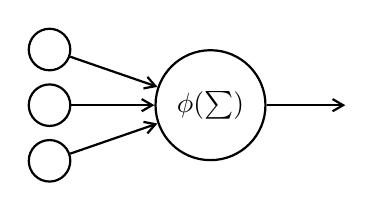
\begin{tikzpicture}
	
	\node[neuron] (a) {};
	\node[neuron,below=of a] (b) {};
	\node[neuron,below=of b] (c) {};
	
	\node[neuron,right=of b] (root) {$\phi(\sum)$};
	
	\node[right=of root] (out) {};

	\node[group,fit={(a) (b) (c)}] (gr1) {};
	\draw[conn] (a) -- (root);
	\draw[conn] (b) -- (root);
	\draw[conn] (c) -- (root);
	\draw[conn] (root) -- (out);

\end{tikzpicture}

	\caption{Neuron mit Eingang, Kernfunktion, Aktivierungsfunktion}
	\label{fig:Neuron}
\end{figure}

Ein Neuron wurde einer Nervenzelle in einem Gehirn mit den folgenden Bestandteilen nachempfunden:
\paragraph{Informationseingangsstrom} ist der Dateneingang, wobei ein Neuron ein bis theoretisch beliebig viele solcher Eingänge haben kann. 
Dies hängt von der jeweiligen Architektur des Netzwerks ab.

\paragraph{Informationsgewichtung} bezeichnet die Gewichtung mit der der Eingangsstrom gewertet wird. 
So wird ein Informationseingangsstrom mehr oder weniger berücksichtigt. 
Diese Gewichtung wird durch den Backpropaga-tion-Algorithmus angepasst und nachjustiert.

\paragraph{Kernfunktion} bewirkt das Verarbeiten der gewichteten Informationseingänge. 
Im einfachsten Fall werden alle Werte aufsummiert. 
Es wäre aber möglich, jegliche Berechnung hier einfließen zu lassen, welche mehrere Werte verwendet und daraus einen neuen Wert berechnet.

\paragraph{Aktivierungsfunktion} berechnet den Ausgang eines Neurons. 
Dabei wird eine weitere Funktion auf das im Kern berechnete Ergebnis ausgeführt, das dazu führt, dass ein Ergebnis noch stärker ausgeprägt weitergegeben wird oder minimiert wird, beziehungsweise in einen Wertebereich eingepasst wird. 
Diese Aktivierungsfunktion ist meist die Sigmoid-Funktion oder eine lineare Funktion, welche in der Abbildung \ref{fig:Aktivierungsfunktion} zu erkennen sind.

\begin{figure}[ht!]
\centering
\subfloat{
\resizebox {0.5\linewidth} {5cm} {
	\begin{tikzpicture}
	\begin{axis}

		\addplot[blue, no markers] expression { 1/(1+exp(-x) };c

	\end{axis}
	\end{tikzpicture}
}
}
\subfloat{
\resizebox {0.5\linewidth} {5cm} {
	\begin{tikzpicture}
	\begin{axis} [xmin=-1, xmax=1]

		\addplot[blue, no markers] expression { x };

	\end{axis}
	\end{tikzpicture}
}
}
	\caption{Basisaktivierungsfunktionen: (l) eine Sigmoid-Funktion, (r) eine lineare Funktion}
	\label{fig:Aktivierungsfunktion}
\end{figure}

\noindent 
Die einfachste Repräsentation eines Neurons lässt sich mathematisch folgendermaßen darstellen.
Im Kern wird eine Summenberechnung durchgeführt. 
Dabei werden die Eingangswerte und deren Gewichtung miteinander multipliziert, sowie diese Ergebnisse aufsummiert.
Der griechische Buchstabe $\phi$ (phi) steht für die Aktivierungsfunktion des Neurons und stellt damit die Ausgabe des Neurons dar.
\begin{equation}
	f(x, w) := \phi ( \sum\limits_{i}{w_i * x_i})
	\label{eq:Aktivierungsfunktion}
\end{equation}

\paragraph{Bias Neuron} 
\label{sec:Bias Neuron}
definiert einen Spezialfall eines Neurons, welches keine Dateneingänge und somit auch keine Gewichtung hat und keine Berechnung im Kern durchführt. 
Dieses liefert nur einen konstanten Wert, wie zum Beispiel eine $1$. 
Durch die konstante Auslieferung wird auch die Aktivierungsfunktion überflüssig. 
Das Bias Neuron stellt somit einen stetigen Wert für das Netzwerk dar, beziehungsweise für die darauffolgende Ebene.

\section{Ebenen/Layer}
\label{sec:Layer}

Ebenen sind Zusammenschlüsse von Neuronen, welche sich auf derselben Stufe befinden. 
Diese Neuronen sind aber nicht miteinander verbunden, sondern bekommen Daten aus der Ebene davor und geben diese an die darauffolgende Ebene weiter. 
Dieser Typ wird \textbf{Hiddenlayer} bezeichnet. 
Jedes Netzwerk benötigt zusätzlich zwei weitere Ausprägungen an Ebenen. 
Diese sind:

\paragraph{Inputlayer} stellt den Übergang zwischen der Welt außerhalb des Neuronalen Netzwerks und dem Netzwerk dar.
Diese Ebene nimmt die Daten ohne Gewichtung auf und gibt sie an die darauffolgende Ebene weiter. 

\paragraph{Outputlayer} befindet sich am Ende eines Netzwerkes. 
Dieser Layer hat die Aufgabe, die Daten nach außen, oder an das darauffolgende Netzwerk weiterzugeben. 
Hierbei werden die Informationen meist nur mehr für die Ausgabe aufbereitet. 
In manchen Netzwerken existieren keine Outputlayer in diesem Sinne, sondern ein Layer, der als Hiddenlayer und Outputlayer fungiert. 
Dies ist der Fall, wenn nur zwei Layer sich im Netzwerk befinden und einer davon vom Inputlayer eingenommen wird.
\\

\begin{figure}
\centering

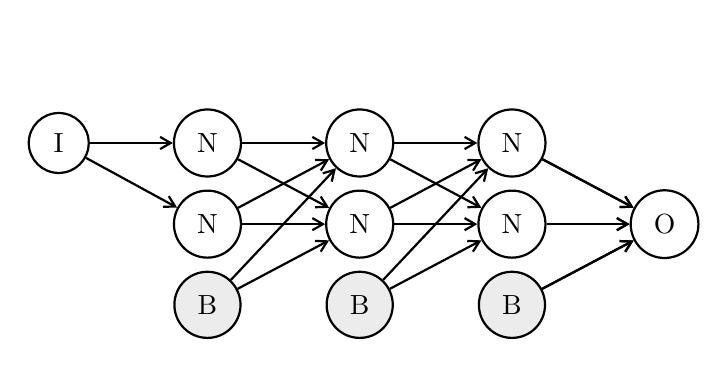
\begin{tikzpicture}

	\node[neuron] (in) {I};

	\node[neuron,right=of in] (1a) {N};
	\node[neuron,below=of 1a] (1b) {N};
	\node[io,below=of 1b] (b1) {B};
	
	\node[group,fit={(1a) (1b) (b1)},right=of in] (gr1) {};
	
	\node[neuron,right=of 1a] (2a) {N};
	\node[neuron,below=of 2a] (2b) {N};
	\node[io,below=of 2b] (b2) {B};
	
	\node[group,fit={(2a) (2b) (b2)},right=of 1a] (gr2) {};
	
	\node[neuron,right=of 2a] (3a) {N};
	\node[neuron,below=of 3a] (3b) {N};
	\node[io,below=of 3b] (b3) {B};
	
	\node[group,fit={(3a) (3b) (b3)},right=of 2a] (gr3) {};
	
	\node[neuron,right=of 3b] (out) {O};
	
	\draw[conn] (in) -- (1a);
	\draw[conn] (in) -- (1b);

	\draw[conn] (1a) -- (2a);
	\draw[conn] (1a) -- (2b);
	
	\draw[conn] (1b) -- (2a);
	\draw[conn] (1b) -- (2b);

	\draw[conn] (b1) -- (2a);
	\draw[conn] (b1) -- (2b);
	
	
	\draw[conn] (2a) -- (3a);
	\draw[conn] (2a) -- (3b);
	
	\draw[conn] (2b) -- (3a);
	\draw[conn] (2b) -- (3b);

	\draw[conn] (b2) -- (3a);
	\draw[conn] (b2) -- (3b);
	
	
	\draw[conn] (3a) -- (out);
	\draw[conn] (3a) -- (out);
	
	\draw[conn] (3b) -- (out);
	\draw[conn] (3b) -- (out);

	\draw[conn] (b3) -- (out);
	\draw[conn] (b3) -- (out);

\end{tikzpicture}

	\caption{Einfaches Neuronales FeedFordward Netzwerk}
	\label{fig:SimpleFeedForwardNetwork}
\end{figure}
\phantom \newline

\noindent 
In der Abbildung \ref{fig:SimpleFeedForwardNetwork} ist ein einfachen FeedFordward Netzwerk abgebildet.
Dieses beinhaltet alle Typen mit Input-, Outputlayer und voll vernetzte Layer mit Neuronen und Bias Neuron. 

\section{Informationen Merken und Wiedererkennung}

Durch das Anpassen der Gewichtungen bei jedem Dateneingangsstrom mit Hilfe des Backpropagation-Algorithmus ist es möglich, Zustände zu speichern und diese auch zu merken. 
Sollte ein ähnlicher Dateneingang stattfinden, wo zuvor schon einer vorhanden war, dann sollte dieser ähnlich behandelt werden.
Dieser kann möglicherweise zu derselben Kategorie gehören, wie der zuvor schon bekannt gemachte und gelernte Dateneingang.

\section{Konvergieren im Maschinellen Lernen}
\label{sec:Konvergieren}

Konvergieren im Maschinellen Lernen bezeichnet das Minimieren der Fehlerquote gegen $0$.
Die Fehlerquote wird dabei als Error bezeichnet und ist ausschlaggebend für den Lernprozess.
Ein Error von $0$ würde bedeuten, dass das Netzwerk keinen Fehler machen würde.
Für die Feststellung des Fehlers gibt es diverse Funktionen, wie zum Beispiel die 'Mean-Square-Error'-Methode.

\section{Backpropagation}
\label{sec:Backpropagation}

Bis zum Jahre 1986 gab es keine automatisierte Möglichkeit, die Gewichtungen in einem Netzwerk automatisch anzupassen.
In diesem Jahre entwickelten Rumelhart, Hinton \& Williams eine mögliche Lösung, welche sehr ähnlich zu anderen Ansätzen von früher war \cite{hecht1988theory}.
Die zentrale Idee in ihrer Lösung liegt darin, die Abweichung des produzierten Ergebnisses zum wirklich erwarteten Ergebnis zu bestimmen. 
Aufgrund dieses Fehlers lassen sich im Anschluss die Gewichtungen im Netzwerk vom Ende zum Anfang nachjustieren. 
Diese Technik ermöglichte damit Netzwerke mit verschachtelten Schichten zu konstruieren und auch zu trainieren.

\paragraph{Lernrate} skaliert den Lernprozess, mit der Auswirkung, ob schneller oder langsamer gelernt wird.
Eine Lernrate unter $0$ würde die Lerngeschwindigkeit stark verlangsamen und ist somit nicht sinnvoll. 
Ein Wert über $1$ würde eine hohe Lerngeschwindigkeit zur Folge haben. 
Eine zu hohe Rate würde nicht zum Konvergieren führen, sondern zum Springen.

\paragraph{Momentum} stellt wie die Lernrate eine Skalierung des Lernprozesses dar.
Dabei werden mit dem definierten Faktor die früheren Gewichtsupdates berücksichtigt. 
Dies führt dazu, dass lokale Tiefpunkte überwunden werden können und das System doch zum globalen Tiefpunkt konvergiert.

\section{Trainieren}

\paragraph{Überwachtes Trainieren} definiert, dass die Daten, welche zur Verfügung stehen aus zwei Teilen bestehen.
Erstens aus den Daten selbst, aus welchen gelernt und verstanden werden soll.
Zweitens aus den Ergebnissen, zu welchen das Netzwerk kommen sollte, welche meistens als Lable bezeichnet werden. 
In dieser Situation liefert das Netzwerk ein Ergebnis, welches mit dem erwarteten Wert verglichen werden kann.
Dieser Unterschied wird zum Feststellen des Fehlers verwendet, welcher besagt, wie inkorrekt das Ergebnis ist.
Des Weiteren wird dieser Fehlerwert für die Backpropagation benötigt.

\paragraph{Unüberwachtes Trainieren} kommt dann zu tragen, wenn nur Daten zum Trainieren zur Verfügung stehen.
Der erwartete Ausgang ist unbekannt.
Diese Strategie wird in Fällen von Clustering (\ref{subsec:Clustering}) verwendet.
Dabei sollen nicht bekannte Gruppen von zusammengehörenden Daten identifiziert werden. 
Self-Organizing Maps (\ref{subsec:SelfOrganizingMap}) entdecken zusammengehörende Muster und geben diese in einer Grafik zur weiteren Interpretation weiter. 
Diese Technik ist insbesonders interessant, da einem Netzwerk nie erklärt worden ist, warum etwas so ist. 
Es steht damit in Relation zu einem natürlichen Lernprozess, wie bei einem Menschen.

\section{Allgemeine Probleme}
\label{sec:AllgeProb}

Ein Grundsatz von neuronalen Netzwerken ist, dass sie nicht jede Frage dieser Welt beantworten können, sondern nur dies durchführen, wofür sie konstruiert wurden. 
Das Entwickeln eines neuen Netzwerks ist eine sehr schwierige und eine lang andauernde Aufgabe. 
Dabei können Fehler auftreten, wie Overfitting, aber auch vom Entwickler verursacht sein können. \\

\noindent
Diese Arbeit wird auf die bekanntesten Probleme eingehen und auch Lösungen oder mögliche Lösungsansätze beinhalten. 

\paragraph{Overfitting} bezeichnet ein Problem, welches nicht nur maschinelles Lernen betrifft, sondern auch Menschen und andere Lebewesen. 
Ein Student lernt zum Beispiel für eine Prüfung und ist im Besitz einer Klausur aus einem Vorjahr. 
Nach öfterem Durchspielen der Fragen und laufenden Selbsttests, befindet er sich in der Lage diese Klausur mit einer sehr hohen Wahrscheinlichkeit zu bestehen. 
Dabei hat sich die Klausur in seinem Gehirn eingeprägt, aber nicht das Stoffgebiet zu welchem er eine Klausur schreiben muss. 
Das Problem wird als Overfitting bezeichnet und beschreibt, dass etwas gemerkt wurde, aber nicht gelernt worden ist und somit eine Abwandlung von Informationen nicht wiedererkannt wird.

\paragraph{Daten} die zum Trainieren von Netzwerken verwendet werden, können selbst ein Problem darstellen.
Eine zu geringe Menge an Daten stellt den Entwickler vor das Problem, dass er für diese Daten ein akkurates Netzwerk entwickeln kann, dieses aber im weiteren Verlauf nicht die gewünschten Resultate liefern wird.
Zusätzlich kann es sein, dass die zur Verfügung gestellten Daten selbst nicht vollständig sind und somit wieder nur ein Subset verwendet werden kann. \\

\section{Domänenklassen}
\label{sec:Domänenklassen}

Neuronale Netzwerke können sehr vielseitig eingesetzt werden. 
Grundsätzlich lässt sich jedes Problem, welches als Funktion repräsentiert werden kann, durch ein Neuronales Netzwerk approximieren. \\

\noindent
In dieser Arbeit werden sieben Hauptdomänen erklärt und beschrieben, welche von Heaton \cite{AI3} definiert wurden. 

\subsection{Clustering}
\label{subsec:Clustering}

Das Clustering Problem bezeichnet das Einordnen von Daten in Klassen oder Gruppierungen. 
Diese Gruppierungen können von einem Netzwerk selbst definiert werden oder manuell festgelegt werden. 
Im Falle einer Self-Organiz-ing-Map werden die Gruppierungen selbst durch das System festgelegt.

\subsection{Regression}
\label{subsec:Regression}

Regression beschreibt den Fall, in welchem Rohdaten generiert werden und diese so verwendet werden. 
Dies kann im Sinne einer Klassifikation verstanden werden mit dem Unterschied, dass die Anzahl der Klassen unendlich ist, wie die der Reellen Zahlen von $[0 - 1]$. 
Ein Anwendungsfall ist das Finden einer zugrundeliegenden Funktion, bei der nur Resultate dieser Funktion vorliegen. 
So gibt es Abläufe in der Natur, welche schwer in einer Funktion festgehalten werden können. 
In diesem Fall lässt sich ein Netzwerk mit den Aktionen und Reaktionen trainieren und erhält eine Approximation der Vorgänge \cite{bishop2006pattern}.

\subsection{Klassifikation}
\label{subsec:Classification}

Bei der Klassifikation werden die Ergebnisse einer Regression, welche meist als Gleitkommazahl vorliegen, auf eine bestimmte Anzahl an Klassen übertragen. 
Der Unterschied liegt im Ergebnis, welches produziert wird.  
Hier werden Daten dem Netzwerk übergeben und dieses muss vorhersagen, zu welcher Klasse sie gehören. Dies wird in einer überwachten Umgebung durchgeführt. 
Die Klassen für die Vorhersage sind vorab schon bekannt und können mit den Daten aus dem Outputlayer des Netzwerks verglichen werden und infolge Justierungen durchgeführt werden \cite{AI3}. \\

\noindent
Ergebnisse einer Klassifikation sagen aus, mit welchem prozentualen Anteil etwas auf den gegebenen Input zutrifft. 
Das Gesamtergebnis ergibt immer 100 Prozent. 
Das Ergebnis bei einer Regression wird dabei nicht in Prozent angegeben, sondern stellt einen konkreten Wert dar.

\subsection{Predict}
\label{subsec:Predict}

Predict-Problemstellungen kommen im Kontext von Business, beziehungsweise von E-Business zur Anwendung. 
Hier muss anhand von meist zeitgesteuerten Ereignissen eine Vorhersage getroffen werden. 
Zum Beispiel an der Börse ändern sich täglich die Kurse relativ rasch, sodass es für Menschen praktisch nicht mehr möglich ist, diese zu verfolgen. 
Im Falle der Börse sind Aktienkurse mit zeitlichem Verlauf aus der Vergangenheit verfügbar. 
Diese können als Trainingsdaten für ein Netzwerk verwendet werden, um den nächsten Tag möglicherweise vorherzusagen. 

\subsection{Robotics}
\label{subsec:Robotics}

Auch bekannt unter dem Namen Robot-Learning. 
Dabei lernen Roboter eigenständig neue Techniken oder passen sich automatisch ihrer Umgebung an. 
Eines der Kernprobleme dabei ist, dass in Echtzeit etwas zur selben Zeit gelernt werden muss, aber auch Aktionen eingeleitet werden müssen, wie das Steuern von Motoren, um zum Beispiel nicht umzufallen.

\subsection{Computer Vision}
\label{subsec:Cumputer Vision}

Computer Vision zielt darauf ab, einem Computer das Sehen und Verstehen von Bildern zu ermöglichen. 
Diese Technik findet im Jahr 2016 schon häufig Einsatz. 
So werden automatisiert Bilder analysiert, beschrieben sowie auch in Gruppen nach diversen Kategorien eingeordnet, wie zum Beispiel nach Gesichtsausdrücken.
Solche Dienste werden auch kommerziell eingesetzt und angeboten. 
In autonom gesteuerten Fahrzeugen findet diese Technologie bereits Verwendung, um Objekte zu erkennen und zu verstehen. 
So muss zum Beispiel ein Verkehrszeichen von einem Passanten unterschieden werden können.

\section{Neuronale Netzwerktypen}

In den letzten Jahren haben sich diverse gut funktionierende neuronale Netzwerktypen gebildet, beziehungsweise sind entwickelt und erforscht worden. 
Diese Netzwerktypen definieren Richtlinien oder Ansätze zu möglichen Netzwerken, welche aber nicht komplett übernommen werden müssen, sondern einen kreativen Spielraum ermöglichen. \\

\subsection{FeedForward}
\label{subsec:FeedForward}

FeedForward Netzwerke (FFN) waren bis vor einigen Jahren noch der Stand der Forschung.
Auf ihnen basieren einige andere Typen von Netzwerken, die bekanntesten werden in dieser Arbeit noch behandelt.
Ein FFN basiert auf den Grundlagen eines Neurons, sowie ihrem Ausbau zu Ebenen mit mehreren Neuronen.
So ein Netzwerk besitzt einen Inputlayer, einen Hiddenlayer sowie einen Outputlayer.
Sobald das Netzwerk eine große Anzahl an Hiddenlayer aufweist, wird es als Deep FeedForward Netzwerk (\ref{subsec:DeepFeedForward}) bezeichnet.
Das FFN weist dabei eine Charakteristik auf, in der der Datenfluss eindeutig definiert ist. 
Der Datenfluss beginnt beim Inputlayer und endet beim Outputlayer, ohne dass ein Datenrückfluss zum Beispiel vom Hiddenlayer in den vorhergehenden Hiddenlayer vorhanden ist.
Dies würde einer Rekursion oder einem Kurzzeitgedächtnis entsprechen.
Die einzelnen Ebenen müssen dabei aber nicht voll verbunden sein, die Vernetzung kann selbst bestimmt werden.

\subsection{Self-Organizing Map}
\label{subsec:SelfOrganizingMap}

Self-Organizing Map (SOM) findet vor allem im Bereich der Classification Verwendung und wurde von Kohonen (1988) erfunden. 
Es ist nicht erforderlich einer SOM die Information zu geben, in wie viele Gruppen oder Klassen die Daten unterteilt werden sollen. 
Dadurch gehört sie zu den Systemen, welche unsupervised trainiert werden. 
Außerdem besitzen sie die Möglichkeit, neue Daten weiter zu klassifizieren und dies über die Trainingsphase hinaus. 
Kohonen entwarf die SOM mit zwei Ebenen, einem Inputlayer und einem Outputlayer ohne Hiddenlayer. 
Der Inputlayer propagiert Muster an den Outputlayer, wo der Dateneingang gewichtet wird. 
Im Outputlayer gewinnt das Neuron, welches den geringsten Abstand zu den Eingangsdaten hat.
Dies geschieht durch das Berechnen der euklidischen Distanz. 
Diese Art von Netzwerk kommt ohne Bias Neuron aus und es kommen ausschließlich lineare Aktivierungsfunktionen zur Verwendung.


\subsection{Hopfield Neuronal Network}

Ein Hopfield Neuronal Network (HNN) \cite{demuth2014neural} ist ein einfaches Netzwerk, welches aus einem Layer besteht. 
In diesem Layer sind alle Neuronen mit jedem anderen Neuron verbunden. 
Dieses Muster wurde von Hopfield (1982) erfunden. 
Im Gegensatz zu anderen Netzwerken können Hopfield Netzwerke in einer Matrix abgebildet werden, in welcher die Gewichtung zu den einzelnen Neuronen abgebildet werden. 
Das Problem bei diesem Typ ist, dass jedes Neuron auf dem Status des anderen aufbaut.
Dies stellt ein Problem für die Reihenfolge der Berechnung dar, was zu einem nicht stabilen Zustand führt.
Durch das Hinzugeben einer Energiefunktion kann festgestellt werden, in welchem Zustand sich das Netzwerk befindet. 
Hiermit kann ein Haltepunkt definiert werden, ab welchem keine Trainingsiteration mehr durchlaufen werden soll. 

\subsection{Boltzmann Machine}

Im Jahre 1985 stellten Hinton \& Sejnowski \cite{Hinton:Boltzman:2007} das erste Mal eine Boltzmann Maschine vor.
Es stellt ein Zwei-Ebenensystem dar, mit einem Inputlayer und einem Outputlayer, wo jeder Knoten mit jedem verbunden ist, außer mit sich selbst.
Das voll vernetzte System unterscheidet eine Boltzmann Maschine von einer eingeschränkten Boltzmann Maschine (RBM), welche eine Grundlage für tiefes Lernen und tiefe Neuronale Netzwerke darstellt.
In einer RBM sind alle sichtbaren Neuronen mit allen Neuronen im Outputlayer verbunden. 
Die Verbindungen zwischen den Neuronen im selben Layer entfallen.
Der alte uneingeschränkte Typ der Boltzmann Maschinen eignet sich gut für Optimierungsprobleme sowie für Mustererkennungen.

\subsection{Deep FeedForward}
\label{subsec:DeepFeedForward}

Deep FeedForward Netzwerke unterscheiden sich von den normalen FeedForward Netzwerken in dem, dass sie mehrere Hiddenlayer beinhalten anstatt nur einem.

\subsection{NEAT}

NeuroEvolution of Augmenting Topologies (NEAT) Netzwerke sind relativ jung, wobei NEAT für einen Algorithmus steht, der Neuronale Netzwerke entwickelt.
Er wurde von Stanley und Miikkulainen (2002) entwickelt. 
Dieser Typ verwendet genetische Algorithmen, um die Struktur und die Gewichtungen im Netzwerk zu optimieren.
Die Input- und Outputlayer sind identisch mit einem FeedForward Netzwerk.
Dafür fehlt diesem Typ eine innere Struktur. 
Die Verbindungen sind lose, nicht klar definiert und können während dem Trainieren entfernt werden, aber auch wieder hinzugefügt werden.

\subsection{Convolutional Neural Network}

Convolutional Neural Network werden selbst nicht als komplettes eigenes Netzwerk verwendet, sondern in FeedForward Netzwerken.
Im Speziellen, wenn es um Bilderkennung geht.
Dabei werden zwei Ebenen nicht voll vernetzt sondern nur teilweise und somit Gewichtungen eingespart.
Außerdem können die Gewichtungen geteilt werden, sodass immer in dieselbe Richtung verlaufende Verbindungen dieselbe Gewichtung aufweisen.
Dies ermöglicht es, komplexe Strukturen zu speichern und trotzdem die Speicherauslastung niedrig zu halten und die Effektivität aufrecht zu halten.

\subsection{Recurrent Network}

Recurrent Network sind Netzwerke, die nicht nur einen Kontrollfluss haben, sondern auch Rekursionen beinhalten. 
Diese Rekursionen können jedes andere Neuron ansprechen, ausgenommen der Neuronen im Inputlayer.
Ein Problem durch Rekursionen sind Endlosschleifen, welche behandelt werden müssen.
So können Kontext-Neuronen verwendet werden, aber auch eine definierte Anzahl an Iterationen durchlaufen werden, damit die Rekursion nicht mehr fortgeführt wird. 
Eine weitere Option ist so lange zu warten, bis sich die Ausgabe des Neurons stabilisiert hat und sich nicht mehr ändert.
Das Kontext-Neuron nimmt dabei die Stelle eines kurzen Speichers ein, wo ein Zustand für die nächste Iteration zwischengespeichert wird.
Die Informationen, die in einem solchen Neuron gespeichert werden, werden bei diesem Speichervorgang nicht gewichtet, sondern erst, wenn diese Informationen an das Netzwerk zurückgegeben werden.
Diese Rekursionen werden vor allem in Fällen verwendet, wenn es um zeitliche Abläufe und Änderungen geht, wie zum Beispiel bei der Temperatur für den nächsten Tag, hierfür stehen etliche Daten vorangegangener Jahre zur Verfügung.

\paragraph{Elman Network} wurde im Jahre 1990 vorgestellt, sie verwenden Rekursionen mit Kontext-Neuronen. 
Dabei existieren zwei Hiddenlayer mit einem Layer für normale Neuronen und einem mit Kontext-Neuronen. 
Die Kontext-Neuronen sind dabei voll mit dem Hiddenlayer verbunden und dieser gibt die Informationen ungewichtet an die Kontext-Neuronen weiter.
In diesem System existieren so viele Kontext-Neuronen wie Neuronen im Hiddenlayer, sodass jedes Neuron dort ein Kontext-Neuron mit dem neuen Status befüllt.

\paragraph{Jordan Network} wurde 1993 der Öffentlichkeit präsentiert.
Sie sind den Elman Netzwerken sehr ähnlich. 
Es werden wieder Kontext-Neuronen für das Zwischenspeichern verwendet, nur wird dieser Zustand durch den Outputlayer definiert.
So wird der Ausgang gespeichert und in der nächsten Iteration wieder verwendet.
Das Kontext-Neuron ist dabei nur mit dem Outputlayer wieder verbunden und nicht mit einem Hiddenlayer.

\section{Domänen und Typen Matrix}

\begin{figure}
	\includegraphics[scale=0.68]{images/typen_domains.png}
	\caption{Domänen zu Typen Matrix \cite{AI3}}
	\label{fig:DomainMatrix}
\end{figure}

Wie in Abbildung \ref{fig:DomainMatrix} erkennbar ist, existiert kein Netzwerkgrundtyp, der für alle Problemdomänen geeignet ist.
Dies führt zu der Schlussfolgerung, dass je nach Aufgabe und Ziel ein entsprechendes Grundgerüst gewählt werden muss. 
Auf Basis dieses Grundgerüsts können uneingeschränkt weitere Eigenheiten aus anderen Netzwerken eingebaut werden.
In der Praxis findet man selten ein Netzwerk von nur einem Typ für eine größere Problemstellung. 
Das Problem wird auf mehrere kleinere Problemstellungen herabgebrochen, welche hintereinander und teilweise parallel gelöst werden.
Dabei übernimmt jedes Teilnetzwerk eine kleine Aufgabe des Gesamten und zwar die eine, für die es entwickelt wurde. 
Aktuelle Netzwerke wie das 'Inception v3' Netzwerk von Google Research benötigen zwei Wochen mit acht Grafikkarten zum Trainieren. 
Ab diesem Zeitpunkt ist es im Stande, akkurate Resultate zu liefern. 
Dieses Netzwerk ist sehr komplex und besteht nicht nur aus 3 Ebenen, was zur Schlussfolgerung führt, dass je tiefer das Netzwerk ist, desto aufwändiger ist es zu trainieren.

\section{Optimierung}

Optimierungen beeinflussen das Lernverhalten und das Speicherverhalten eines Netzwerkes.

\paragraph{Lernrate} skaliert die Lerngeschwindigkeit, wie im Punkt Backpropagation beschrieben.

\paragraph{Momentum} gehört auch zur Optimierung im Algorithmus zur Backpropa-gation.
Dieser bestimmt wie stark frühere Gewichtsaktualisierungen berücksichtigt werden sollen. 

\paragraph{DropOut} gehört zur Kategorie der Regulatoren. 
Hinton \cite{krizhevsky2012imagenet} beschreibt DropOuts als eine effektive Art, um Overfitting zu vermeiden.
DropOut kann als System integriert werden, aber auch als eigener Layer in einem Netzwerk.
In einem DropOutlayer werden immer Neuronen deaktiviert, inklusive ihrer Verbindungen zum nächsten Layer.
Dies hat zur Folge, dass nur ein geringerer Teil an Informationen aus dem vorhergehenden Layer in den nächsten übergeht. 
Der Prozess des künstlichen Geringhaltens von Informationen während des Trainings führt dazu, dass das Netzwerk trotz dieser Einschränkung versucht, ein gutes Ergebnis zu erzielen. 
Während der Test- und Produktivphase werden diese DropOutlayer aber meist deaktiviert, da das volle Potenzial des Netzwerks verwendet werden soll.

\paragraph{L1 und L2 Regularisierung} sind ebenfalls Techniken, die zur Verhinderung von Overfitting beitragen.
Im Gegensatz zu der DropOut Strategie sind diese zwei Regularisierungstechniken Teil der Backpropagation oder werden als Funktion eingesetzt.
Beide Techniken arbeiten mit Strafen, welche verteilt werden und so die Gewichtungen vor dem Ausarten hindern. 
Durch das Bestrafen der Gewichtungen im Netzwerk werden diese Werte gering gehalten. 
Wenn ein Gewicht Richtung $0$ geht, führt dies unweigerlich zu einem indirekten Ausschluss aus dem Netzwerk. 
Das Netzwerk wird spärlicher und leichtgewichtiger, sodass ein Rauschen in den Daten ignoriert wird. 

\begin{equation}
	E := \frac{\lambda}{n} \sum |w|
	\label{eq:L1ErrorTerm}
\end{equation}

\noindent
Die Funktion \ref{eq:L1ErrorTerm} bildet die Berechnung der Strafe in der Backpropagation ab.
Das $\lambda$ definiert wie stark die Regularisierung den Error-Wert des Netzwerkes beeinflussen soll.
Ein Wert von $0$ führt dazu, dass die Regularisierung keinen Einfluss besitzt. 
Im einem normalen Fall ist dieser Wert kleiner als $0.1 (10\%)$.
Der Divisor n wird durch die Anzahl an Elementen im Trainingssatz und der Anzahl an Neuronen im Outputlayer bestimmt.
Zum Beispiel bei $100$ Elementen im Trainingssatz und $3$ Neuronen im Outputlayer würde der Divisor den Wert $300$ einnehmen.
Dies ist erforderlich, da diese Funktion bei jeder Evaluierung der Trainingsdaten berechnet wird.

\section{Trainingsgeschwindigkeitssteigerung}

\paragraph{GPU - GPGPU} ist die Bezeichnung für die Verwendung des Grafikprozessors über seine ursprüngliche Auslegung darüber hinaus.
In der aktuellen Zeit ist es nicht mehr möglich, eine Geschwindigkeitssteigerung zu erreichen, indem die Taktrate des Prozessors erhöht wird. 
Deshalb wird mehr parallelisiert, da die Recheneinheiten kleiner werden und so mehrere auf derselben Fläche Platz finden. 
Eine Grafikkarte besitzt die Eigenschaft, gleichförmige Operationen in einem Schritt auf sehr viele Objekte gleichzeitig auszuführen. 
So werden viele Pixel auf einmal eingefärbt oder eine Multiplikation großer Matrizen durchgeführt. 
Der Geschwindigkeitsvorteil kommt dabei durch den hohen Grad an Parallelität, da die Grafikkarte hauptsächlich für solche Operationen ausgelegt worden ist.

\paragraph{Batch Learning} 
führt dazu, dass immer ein Paket an Daten in das System eingeführt wird. 
Dieses Paket wird je nach Implementierung parallel verarbeitet oder sequenziell. 
Der Unterschied zu 'Online Learning' ist nun, dass nicht nach jedem Datensatz die Gewichtungen und das System nachjustiert wird, sondern dass zuerst das Paket verarbeitet und das System einmal angepasst wird. 
Dabei werden die Gradienten zusammengerechnet und einmal auf den Graphen adaptiert \cite{AI3}. 
\chapter{TensorFlow}
\label{cha:TensorFlow}

TensorFlow repräsentiert eine Bibliothek für Machine Intelligence. 
Historisch gesehen entstand TensorFlow in der Google Brain Abteilung.
Das Projekt wird als Open Source Projekt weiterentwickelt, wobei das Projekt von Google weiterhin gepflegt wird. 
Das Offenlegen des Projekts führt dazu, dass auch Personen außerhalb von Google die Möglichkeit bekommen, die Bibliothek zu verwenden sowie dazu etwas beitragen zu können. \newline

\noindent
Das Hauptkonzept in TensorFlow sind sogenannte Tensoren, welche einen Graphen durchlaufen. 
%Diese Tensoren werden während ihrem durch lauf verändert und wieder neu zusammengesetzt. 
Der Graphen selbst stellt damit einen Datenflussgraphen dar, welcher Knoten beinhaltet. 
Diese Knoten bilden numerische Operationen ab.
Der Informationsaustausch zwischen den Knoten geschieht mit multidimensionalen Arrays, den so genannten Tensoren.
TensorFlow bietet wie andere Bibliotheken die Möglichkeit die Berechnungen auf eine Grafikkarte auszulagern.
Zusätzlich sind weite Routinen eingebaut, damit das Trainieren über mehrere Grafikkarten verteilt werden kann sowie auf weitere Computer. \newline

\noindent
TensorFlow steht für mehrere Programmiersprachen zur Verfügung, welche offiziell unterstützt werden, wobei es noch mehr durch die Open Source Gemeinschaft unterstützte Sprachen gibt.
Den Hauptbereich stellt die Python API dar, welche auch die vollständigste Implementierung darstellt. 
Der Kern von TensorFlow ist mit C++ und Python implementiert und wurde sehr stark optimiert, um eine sehr gute Performanz zu erzielen.
Die Python API wird im Umfeld von TensorFlow dazu verwendet, um einen Graphen zu erstellen, zu trainieren und zu testen. 
Durch die Verwendung von Python besteht die Möglichkeit sehr schnell Änderungen am Graphen durchzuführen und nicht erst ganze Applikationsstrukturen zu übersetzten, damit ein Ergebnis der Änderung ersichtlich wird. 
Dieser Graphen wird nach seiner Trainingsphase exportiert und beinhaltet alle Knoten sowie die dazugehörigen Gewichtungen. 
Die C++ API sowie die Java API und GO API zielen auf eine sehr effiziente Ausführung ab.
Durch die Verwendung des trainierten Graphen kann dieser auch auf mobilen Plattformen eingesetzt werden.

\subsection{Graphs/Dataflowgraph}

\begin{figure}
\lstset{language=Python}
\begin{lstlisting}
import tensorflow as tf

b = tf.Variable(tf.zeros([100])) 
	# 100-d Vektor, initialisiert mit 0
W = tf.Variable(tf.random_uniform([784,100],-1,1)) 
	# 784x100 Matrix w/rnd vals
x = tf.placeholder(name="x") 
	# Platzhalter für Eingangsdaten
relu = tf.nn.relu(tf.matmul(W, x) + b) 
	# Relu(Wx+b) Aktivierungsfunktion mit impliziter Addition
C = [...] 
	# Kostenfunktion und noch weitere Knoten
s = tf.Session()
for step in xrange(0, 10):
	input = ...construct 100-D input array ... 
		# Erstellen eines 100-d Vektor mit den Eingangsdaten
	result = s.run(C, feed_dict={x: input}) 
		# Graphen mit den Eingangsdaten ausführen
	print step, result 
		# Ausgabe des Berechneten Resultats
\end{lstlisting}

	\caption{TensorFlow Codefragment zur Definition eines Teils des Graphen}
	\label{fig:SimpleFragmentGraphDefinition}
\end{figure}
\begin{figure}
	\centering

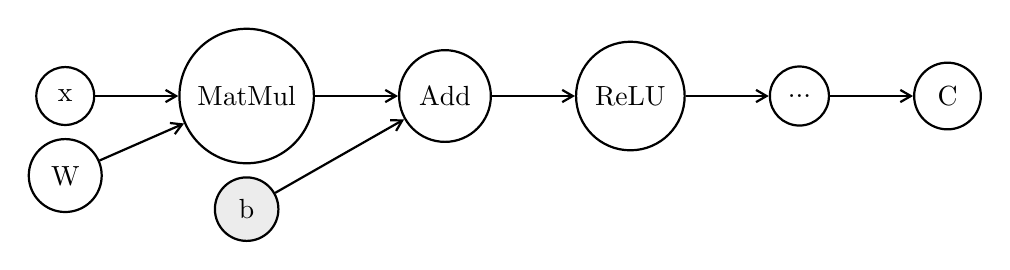
\begin{tikzpicture}

	\node[neuron] (x) {x};
	\node[neuron,below=of x] (w) {W};
	
	\node[group,fit={(x) (w)}] (gr1) {};
	
	\node[neuron,right=of x] (MatMul) {MatMul};
	\node[io,below=of MatMul] (b) {b};
	
	\node[group,fit={(x) (MatMul)},right=of x] (gr2) {};
	
	\node[neuron,right=of MatMul] (Add) {Add};
	
	\node[neuron,right=of Add] (ReLU) {ReLU};
	
	\node[neuron,right=of ReLU] (more) {...};
	
	\node[neuron,right=of more] (C) {C};
	
	\draw[conn] (x) -- (MatMul);
	\draw[conn] (w) -- (MatMul);

	\draw[conn] (MatMul) -- (Add);
	\draw[conn] (b) -- (Add);
	
	\draw[conn] (Add) -- (ReLU);
	\draw[conn] (ReLU) -- (more);

	\draw[conn] (more) -- (C);

\end{tikzpicture}

	\caption{Der resultierenden Teilgraph aus dem Codefragment aus Abbildung \ref{fig:SimpleFragmentGraphDefinition} nach dem Beispiel in \cite{wp2015tensorflow}}
	\label{fig:SimpleFragmentGraphPic}
\end{figure}
Ein TensorFlow Graph kann wie in Abbildung \ref{fig:SimpleFragmentGraphDefinition} beschrieben werden.
Dieser wurde zum Beispiel mit der Python API erstellt.
Im Gesamten mit den Knoten und den Verbindungen ergibt sich ein Datenfluss, diese beinhaltet alle erforderlichen Komponenten auch für das per sistieren und aktualisieren der Daten.
Dies sind Erweiterungen für den Hauptgraphen und beinhalten auch Logik für Schleifenverwaltungen.
Ein Knoten in einem Graphen besitzt $0$ bis $n$ Ein und Ausgänge und besitzt eine Kernfunktion. 
Zu den Datenhauptfluss mit den Tensoren gibt es zusätzlich spezielle Verbindungen, welche "control dependencies" genannt werden. 
Anhand dieser Verbindungen werden keine Daten im Sinne der Tensoren übertragen, sondern werden benützt um Abhängigkeiten zu definieren, um zum Beispiel eine Ausführung in einem anderen Knoten vor einem anderen zu definieren.
So muss der Quellknoten mit der Ausführung abgeschlossen haben bevor der darauf wartende mit der Ausführung beginnt. \cite{wp2015tensorflow}

\subsection{Operation}

Die Operation stellt in jedem Knoten den Kern dar, wie zum Beispiel eine Matrix Multiplikation oder eine Addition.
In TensorFlow selbst gibt es einen Unterschied zwischen Operation und Kernel.
Operationen besitzen Attribute, welche spätestens zum Zeitpunkt der Grapherstellung bekannt sein müssen. 
Ein solches Attribut wäre zum Beispiel, \textit{um eine Operation Polymorph für Datentypen zu ermöglichen}. 
Der Kernel selbst ist die Implementierung der Operation selbst. 
Dieser kann auf verschiedenen Geräten ausgeführt werden wie CPU oder GPU.
Die Operationen und die dazugehörigen Kernel werden über einen Registrierungsmechanismus zur Verfügung gestellt. 
Diese Sammlung an Operationen kann auch Erweitert werden. \cite{wp2015tensorflow} 

\subsection{Sessions}

Die Session repräsentiert die Laufzeit für einen Graphen. 
Dieser Session wird ein Graphen übergeben, welcher erst initialisiert werden muss. 
Ohne die Initialisierung ist der Knoten und Verbindungen würde die weitere Ausführung mit diesem nichts produzieren, da alle Werte $0$ sind. 
Diese stellt eine weitere Funktion zur Verfügung \textit{Run}. 
Der Run-Funktion wird eine Liste Endknoten übergeben welche berechnet werden sollen und die zu dem initialisierten Graphen gehören. 
Die Platzhalter Tensoren werden mit Daten verknüpft und so in den Graphen gereicht. 
In den Meisten fällen wird ein Graphen einmal erstellt und mehrfach ausgeführt. \cite{wp2015tensorflow} 

\subsection{Tensor}

In TensorFlow ist ein Tensor ein typisiertes multidimensionales Array. 
Die verwendbaren Typen reichen von Datentypen mit Vorzeichen und ohne sowie bis hin zu Doubles und Zeichenketten. \cite{wp2015tensorflow} 

\subsection{Hyperparameter} 

Hyperparameter werden im Umfeld von maschinellem Lernen verwendet, um Variationen an Kombinationen zu testen. 
Dabei werden verschiedenste Parameter getestet, wie verschiedene Aktivierungsfunktionen oder Optimierungsalgorithmen, aber auch die Anzahl an Ebenen und Breiten dieser. 
Im Gesamten führt dies meist zu sehr vielen Permutationen, welche ausgetestet werden müssen und somit voll trainiert werden. 
Da die Zeit welche dafür benötigt werden würde, nicht in einer Relation dazu steht, werden solche BroudForce Tests nur mehr selten durchgeführt. 
Für diesen Fall existieren eigene Techniken, welche sich nur um das Optimieren der Hyperparameter kümmern. \cite{bishop2006pattern}

\section{Bibliotheksinhalt}

\subsection{Datentypen}

TensorFlow besitzt eine große Anzahl an Datentypen die verwendet werden können. 
Dies reicht von Grunddatentypen wie 'Boolean' und 'String' bis hinzu verschiedene Integer Datentypen. 
Diese stehen in verschiedene Wertebereichen zur Verfügung. 
So gibt es Gleitkommazahlen mit unterschiedlicher Genauigkeit, wie 16-bit was für halbe Genauigkeit steht aber auch bis zu 64-bit Genauigkeit reicht, was einer doppelten Genauigkeit entspricht. 
Der Grund für diese verschiedenen Anzahlen an Datentypen ist, dass diese zur Optimierung verwendet werden können. 
Ein trainiertes Netzwerk welches nie in den Wertebereich von 64-bit signierte Integers gekommen ist, wird diese möglicherweise nie benötigen. 
In diesem Fall können die Wertebereiche reduziert werden, auf zum Beispiel 32-bit signierte Integer und somit die Berechnungen hochperformanter ausgeführt werden. \cite{TensorFlow}

\subsection{Operationen}

\subsubsection{Konstanten und Zufallswerte}

\paragraph{Konstanten} stehen in TensorFlow vordefiniert zur Verwendung.
Diese stellen initialisierte Tensoren für den ersten Trainingsdurchlauf zur Verfügung.

\begin{itemize}
	\item \textit{tf.zeros} erstellt einen Tensor mit angegebenen Dimension bestehend aus $0$ und von einem Datentypen. 
	\item \textit{tf.zeros\_like} gibt einen Tensor zurück, welcher die selbe Dimensionen wie der gegeben besitzt.
	Alle Werte in diesem Tensor sind aber auf $0$ gesetzt.
	In diesem Zuge kann der Datentyp mit angepasst werden, wenn nur die Dimensionen übernommen wenden sollen.
	\item \textit{tf.ones} agiert genau wie der Tensor \textit{tf.zeros} mit dem unterschied dass alles mit $1$ gefüllt ist.
	\item \textit{tf.ones\_like} repräsentiert das selbe wie \textit{tf.zeros\_like} nur mit $1$.
	\item \textit{tf.fill} wird zu der Dimension noch ein Skalar mit gegeben, für die Werte die ausgefüllt werden sollen.
	\item \textit{tf.constant} liefert einen Tensor mit selbst definierbaren Werten. 
	Diese Werte können eine Liste sein sowohl als auch eine einzelner Wert welcher überall eingefügt werden soll. 
\end{itemize}

\paragraph{Sequenzen} können verwendet werden um einen Wertebereich in eine bestimmte Anzahl an Werte zu zerteilen und diese als Tensor in das System einfließen zu lassen.

\begin{itemize}
	\item \textit{tf.lin\_space} generiert einen eindimensionalen Tensor vom Datentypen $32$ oder $64$-bit Gleitkommazahlen, mit einer bestimmten Folge.
	Diese beginnt mit dem Startwert und endet mit dem Endwert. 
	Die Werte dazwischen werden gleichmäßig verteilt erstellt. 
	\item \textit{tf.range} erstellt wie \textit{tf.lin\_space} einen eindimensionalen Tensor mit Skalarwerten. 
	Die Folge beginnt mit einem Startwert und erweitert sich um ein Delta bis zum Endwert, welcher nicht Teil der Folge ist. 
\end{itemize}

\paragraph{Zufallswerte} werden im Bereich von maschinellen Lernens sehr häufig benötigt. 
So werden meist der Startzustand mithilfe von Zufallszahlen hergestellt. 

\begin{itemize}
	\item \textit{tf.random\_normal} liefert einen Tensor mit Zufallswerten anhand einer Normalverteilung (Gaussian). 
	Die Dimension des Ergebnistensors muss spezifiziert werden, der Meridian, Standardabweichung sowie der resultierende Datentyp können angegeben werden. 
	\item \textit{tf.truncated\_normal} verhält sich gleich zu \textit{tf.random\_normal} mit dem unterschied, dass Werte die größer sind als $2$-mal die Standardabweichung, ignoriert werden und ein neuer Wert ausgewählt wird.
	\item \textit{tf.random\_uniform} generiert einen Tensor in welchem Werte gleich Wahrscheinlich vorkommen.
	Die Werte werden aus dem spezifizierten Wertebereich genommen, wobei diese exklusive der oberen Grenze ist, wie zum Beispiel '$[0, 1)$'.
	\item \textit{tf.random\_shuffle} erstellt selber keine neuen Werte sondern, mischt einen Tensor anhand seiner ersten Dimension durch. 
	\item \textit{tf.random\_crop} liefert einen zufälligen Teil eines Tensors mit der selben Anzahl an Dimensionen und aber mit der spezifizierten Größe.
\end{itemize} \phantom \newline

\noindent
Einige dieser Funktionen benötigen sogenannte Seed-Werte, welche den Startwert der Zufallszahlen zerstreuen sollen sowie die Folge selbst. 
Im Falle von TensorFlow beruht dies auf zwei Werten, einer wird für den Graphen spezifiziert, der zweite wird für die Operation selbst spezifiziert. 
Der Wert für den Graphen kann mit \textit{tf.set\_random\_seed} gesetzt werden. 
Für weiter Informationen steht die online Dokumentation zur Verfügung. \footnote{Online Dokumentation: Constants, Sequences, and Random Values  \url{www.tensorflow.org/api_guides/python/constant_op}}

\subsubsection{Variables}

Variablen geben bei jedem Durchlauf einen Tensor ab.
Dieser Wert ändert sich nicht, außer ihm wird eine neuer Wert zugewiesen. 

\subsubsection{Transformationen}

\paragraph{Casting} bietet die Möglichkeit wie in anderen Programmiersprachen Typen zu konvertieren. 
Diese Operation muss in den Graphen eingepflegt werden, da keine impliziten Konvertierungen durchgeführt werden. 
Es kann jeder Tensor konvertiert werden, sowie eine Zeichenfolge in eine Zahl. 
Bei diesem Vorgang kann ein Fehler entstehen, welcher in \textit{TypeError} resultiert.

\paragraph{Shapes und Shaping} liefert die Gestalt eines Tensors, bietet aber auch die Möglichkeit diese zu ändern. 
\begin{itemize}
	\item \textit{tf.shape} liefert eine genaue Aufschlüsselung des Tensors mit der Dimension und der Tiefe.
	\item \textit{tf.size} repräsentiert die Anzahl an Elementen in einem Tensor. 
	Diese Anzahl ergibst sich aus den konkreten Werten.
	\item \textit{tf.rank} verhält sich ähnlich zu \textit{tf.size} mit dem unterschied, dass die Anzahl der Felder Vertiefung gezählt wird.
	\item \textit{reshape} wird verwendet um Tensoren in eine neue Struktur zu bringen. 
	Dabei kann für das einebnen der Dimensionen eine Kurzschreibweise verwendet werden mit $-1$ als Zielausführung der Gestalt.
	\item \textit{tf.squeeze} entfernt ganze Dimensionen aus dem gegebenen Tensor. 
	Ohne Achsen Angabe werden alle Dimensionen mit der Größe $1$ entfernt oder es werden die spezifizierten Dimensionen herausgenommen.
	\item \textit{tf.expand\_dims} gliedert wider um Dimensionen in einen Tensor ein. 
	Im Standard an der Indexstelle $0$, außer es wurde spezifiziert.
\end{itemize}

\paragraph{Slicing und Joining} wie in diversen Programmiersprachen unterstützt auch TensorFlow das Teilen und Zusammenfügen von Daten und aber hier im Speziellen mit Tensoren. 
Diese Operationen reichen von einfachen Slicing Operationen über Transponieren bis hin zu dem Verketten von Tensoren, dabei kann definiert werde Anhand welcher Achse der Dimensionen die Operation ausgeführt werden soll. 
%\paragraph{Fake quantization} => zu viel
\phantom \newline

\noindent
Weiter Informationen befinden sich in der online Dokumentation. \footnote{Online Dokumentation: Tensor Transformations \url{www.tensorflow.org/api_guides/python/array_ops}}

\subsubsection{Mathematik} 

\paragraph{Arithmetische Operationen} stellen die mathematischen Grundoperationen dar. 
Diese können teilweise in Kurzschreibweisen verwendet werden, wie zum Beispiel die Addition. 
Diese kann entweder als explizite Operation \textit{tf.add(x, y)} verwendet werden aber auch Implizit bei der Addition $+$ von einem Tensor mit einem Bias-Tensor.

\paragraph{Basis Funktionen} ergänzen die arithmetischen Operationen um Standardfunktionen. 
Zu diesen Funktionen zählen die Berechnung der Absolutwerten in einem Tensor sowie eine Exponentialfunktion. 

\paragraph{Matrizen Funktionen} werden am häufigsten benötigt, da Tensoren im Grunde Matrizen sind und somit diese geändert werden können. 
\begin{itemize}
	\item \textit{tf.matmul} führt eine Matrizenmultiplikation aus. 
	Diese Operation findest meist in voll Vernetzten Neuronen Verwendung, wenn der übergebene Tensor mit der Gewichtung multipliziert wird. 
	\item \textit{tf.eye} erzeugt eine Identitätsmatrix, in welcher alle Werte an der Diagonale $1$ sind und alle anderen $0$. 
\end{itemize}

Zu diesen Funktionen existieren noch weitere die zur Lösung von Gleichungen verwendet werden können. 
Diese Gleichungen müssen in Matrizenschreibweise im Tensor abgebildet sein. 

\paragraph{Komplexe Zahlen} können verwendet werden und Operationen mit ihnen in de Graphen eingepflegt werden. 

\paragraph{Reduzierungsoperationen} kommen meist dann zum Einsatz, wenn der Unterschied zwischen dem Ergebnis und dem erwarteten Ergebnis festgestellt werden soll. 
\begin{itemize}
	\item \textit{tf.reduce\_sum} berechnet die Summe aller Werte in einem Tensor.
	\item \textit{tf.reduce\_mean} berechnet die Summe aller Werte an der Diagonale eines Tensors. 
	\item \textit{tf.reduce\_max} reduziert einen Tensor auf die maximal Werte in der letzten Dimension und reduziert dabei den Rang um eins.
\end{itemize}

\noindent
Zu diesen gibt es noch weiter, welche in diversen Fällen benötigt werden wenn zum Beispiel Wahrheitswerten reduziert werden sollen. \newline

\noindent
Die Anzahl an mathematischen Funktionen ist um einiges sehr viel Größer als die hier erwähnten. 
Diese hier repräsentieren lediglich die meist verwendeten Operationen. 
Für weiter Informationen steht die online Dokumentation zur Verfügung. \footnote{Online Dokumentation: Math  \url{www.tensorflow.org/api_guides/python/math_ops}}

\subsubsection{Flusskontrolle}

\paragraph{Flusskontrolle} sind Operationen die den Ablauf in dem Graphen beeinflussen. 
Dies können Bedingungen sein, wie im Sinne von \textit{if (Bedingung){...} else {}} aber auch \textit{switch (Term) { case '0': ...; break;}} Bedingungen sein. 
In beiden Fällen müssen die Auszuführenden Verzweigungen als Funktionen vorliegen. 
Zusätzlich gibt es noch eine \textit{While} und eine \textit{For} Schleife. 
Zu beachten ist, dass diese Operationen und weiter den Fluss durch den Graphen stark beeinträchtigen können.

\paragraph{Logik Operatoren} können verwenden werden um Vergleiche zwischen Tensoren durchzuführen. 
Diese werden aber als Logik Operationen ausgeführt und liefern immer Wahrheitswerte, wie eine Logische Und-Verknüpfung auf Binärebene.

\paragraph{Vergleichsoperatoren} neben den Logischen Operatoren stehen weitere Vergleichsoperatoren zur Verfügung. 
Hierzu zählen \textit{tf.equal} sowie die verneinte Variante, \textit{tf.less} und \textit{tf.greater} mit jeweils einer gleich Version. 
Diese Operatoren geben wiederum einen Tensor mit Wahrheitswert aus.

\paragraph{Debugging Operationen} ermöglichen es in den Graphen Kontrollstrukturen einzubauen, welchen auf diverse Bedingungen reagieren.
So kann Überprüft werden ob ein Tensor Werte mit undefinierten Zustand beinhaltet. 
Die Funktion \textit{tf.Print} ermöglicht es Tensoren auszugeben wenn diese Funktion im Graphen evaluiert wird. 
Aktuell sind die Möglichkeiten eine Graphen zu debuggen relative eingeschränkt, da der Graphen ist grundsätzlich einsehbar aber schwer zu verstehen in seiner rohen Darstellung.
\footnote{Online Dokumentation: Control Flow \url{www.tensorflow.org/api_guides/python/control_flow_ops}}

\subsubsection{Images}

\paragraph{Encodieren und Decodieren} von Bilddateien wird TensorFlow direkt unterstützt.
Dabei können Bildern von den Datentypen Gif, Jpeg und PNG gelesen werden, sowie das erstellen von Bildern in diese Datentypen, ausgenommen Gif. 
In allen Fällen wird das Bild als Zeichenkette mit Pfad angegeben. 

\paragraph{Größenänderung} von Bilder sind erforderlich, da Bilder die eingelesen werde zu große sind und somit in die Struktur des Graphen nicht eingelesen werden können. 
Für die Größenänderung stehen mehrere Implementierungen zur Verfügung mit unterschiedlichen Algorithmen und vorgehen im Hintergrund.

\paragraph{Beschneiden} wird dann benötigt wenn aus einem Bild ein Teil herausgenommen werden soll. 
Zum herausnehmen stehen wiederum mehrere Operationen zur Verfügung, welche mit umschließende Boxen arbeiten oder wie viel Prozent von der Mitte des Bildes aus genommen werden soll.

\paragraph{Flippen, Rotieren und Transponieren} ermöglicht es Bilder zu Verändern, so dass es für einen Menschen mehr oder weniger immer noch die selbe Bedeutung hat aber nicht mehr für einen Computer. 
Für diesen stellt ein Rotiertes oder Gespiegeltes Bild ein neues Bild dar. 
Diese Technik wird beim Trainieren von Bilderkennungen eingesetzt um zum Beispiel aus geringen Datenmengen die zum Trainieren verfügbar sind, mehrere zu generieren.
\phantom \newline

\noindent
Zusätzlich gibt es noch die Möglichkeit die Farbkanäle des Bildes zu ändern sowie das Bild nachzujustieren. 
\footnote{Online Dokumentation: Images \url{www.tensorflow.org/api_guides/python/image}}

\subsubsection{Input und Readers}

\paragraph{Platzhalter} werden benötigt um einen Graphen zu erstellen. 
Ohne Platzhalter wäre es nicht möglich Daten in den Graphen zu bekommen. 
Diese müssen zur Ausführungszeit durch richtige Daten ersetzt werden, was mit Hilfe von einem Schlüssen-Wert-Paars erfolgt. 

\paragraph{Readers} ermöglichen direkt aus dem Dateisystem Daten zu laden. 
Dabei stehen spezifizierte Reader zur Verfügung welche die direkt Tensoren ausliefern sowie Zeile für Zeile  oder ganze Dateiinhalte liefern. 

\paragraph{Konvertierungsoperationen} ermöglichen es Dateien die mit TensorFlow Readers gelesen wurden weiter zu verarbeiten, so kann eine CSV Datei decodiert verwendet werden.
\phantom \newline

\noindent
Des Weiteren sind Protokoll Buffer sowie Queues implementiert die zum Vorverarbeiten von Daten sind.
\footnote{Online Dokumentation: Input und Readers \url{www.tensorflow.org/api_guides/python/io_ops}}

\subsubsection{Neuronale Netzwerke}

Neuronale Netzwerke sind eine Spezialisierung des Gebietes des maschinellen Lernens. 
So bietet TensorFlow eine breite Unterstützung beziehungsweise eine große Implementierungsvielfalt für diesen Typ an. 

\paragraph{Aktivierungsfunktion} repräsentieren den Ausgang eines Neurons dar, dabei existieren aus der Vergangenheit heraus einige Ansätze für diesen Bereich eines Neuronalen Netzwerkes. 
\begin{itemize}
	\item \textit{tf.sigmoid} ist eine der bekanntesten und ältesten diesen Typs.
	Diese Funktion hat im Punkt $0$ einen Aktivierungswert von $0.5$ und besitzt zwei Beschränkungen. 
	Im negativen Zahlenbereich auf der X-Achse wird die Funktion mit $0$ der Grenzwert definiert und im positiven Zahlenbereich auf der X-Achse wird diese mit dem Grenzwert von maximal $1$ definiert. 
	Ein negativer Wert führt somit zu einem geringen Aktivierungswert, welcher sich im Negativen an $0$ annähert sowie im Positiven an $1$.
	Im Diagramm \ref{fig:Sigmoide Aktivierungsfunktion} befindet sich dies Funktion mit ihren Grenzwerten. 
\begin{figure}
	\centering
	\resizebox {\linewidth} {5cm} {
	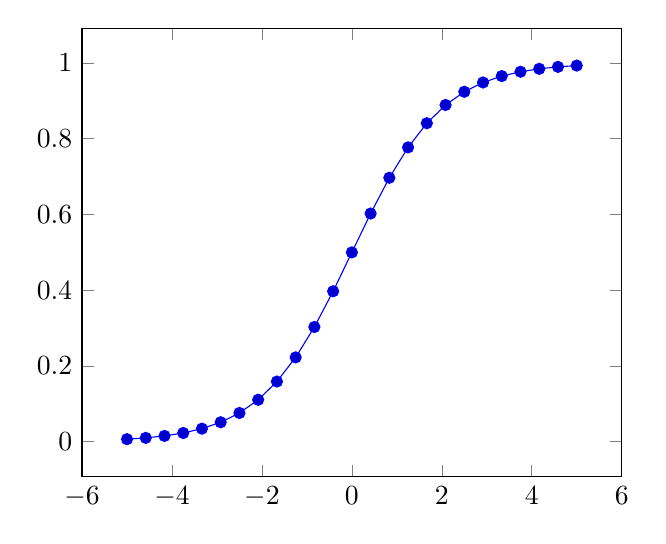
\begin{tikzpicture}
	\begin{axis}

		\addplot expression { 1/(1+exp(-x) };

	\end{axis}
	\end{tikzpicture}
	}
	\caption{Sigmoide Aktivierungsfunktion}
	\label{fig:Sigmoide Aktivierungsfunktion}
\end{figure}
	\item \textit{tf.relu} ersetzt mittlerweile immer mehr die Sigmoide Version. 
	Ein Grund dafür ist, dass die Berechnung mit Sigmoidefunktionen Ressourcen intensive ist. 
	Die rektifiziert lineare Funktion ist sehr viel einfacher, denn Werte unter $0$ werden als $0$ weiter gegeben und Werte darüber linear. 
	Somit resultiert ein Eingangswert von $-0.1$ in einer $0$ und ein Wert von $0.5$ in $0.5$.
	Wie im Diagramm \ref{fig:rektifiziert lineare Aktivierungsfunktion} ersichtlich ist, führt dies bei einem negativen Wert dazu, dass eine Multiplikation mit der Gewichtung in der nächsten Ebene ebenfalls in einer $0$ sich repräsentiert und somit in der Addition ignoriert wird.
\begin{figure}
	\centering
	\resizebox {\linewidth} {5cm} {
	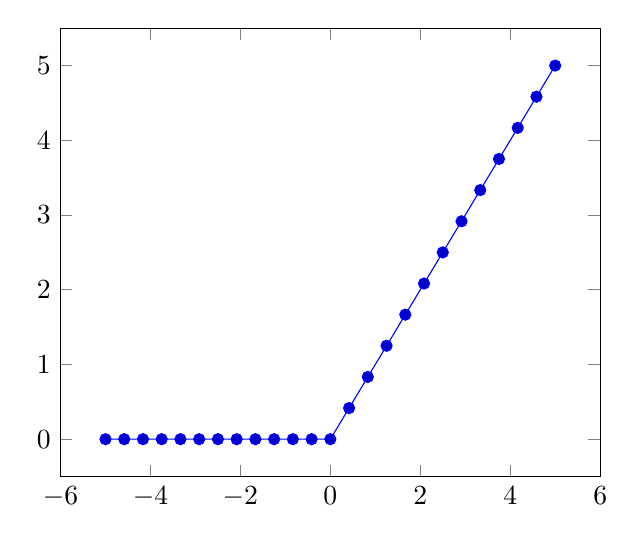
\begin{tikzpicture}
	\begin{axis}

		\addplot expression { max(0, x)};

	\end{axis}
	\end{tikzpicture}
	}
	\caption{rektifiziert lineare Aktivierungsfunktion}
	\label{fig:rektifiziert lineare Aktivierungsfunktion}
\end{figure}
	\item \textit{tf.tanh} genannt als Hyperbolic Tangent gehört ebenfalls zu den grundlegenden Aktivierungsfunktionen. 
	Der Unterschied zwischen dieser Funktion und der Sigmoiden Aktivierungsfunktion ist, dass der untere Grenzwert nicht bei $0$ liegt sondern bei $-1$. 
	Im Diagramm \ref{fig:Hyperbolic Tangents Aktivierungsfunktion} ist zu sehen, wo sich der Wendepunkt befindet, was im Falle des Hyperbolic Tangent in der Koordinate $x = 0, y = 0$ ist. 
\begin{figure}
	\centering
	\resizebox {\linewidth} {5cm} {
	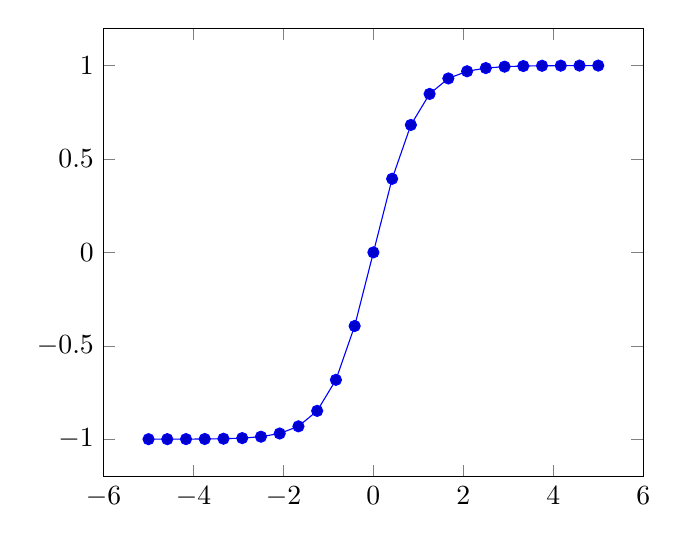
\begin{tikzpicture}
	\begin{axis}

		\addplot expression { tanh(x)};

	\end{axis}
	\end{tikzpicture}
	}
	\caption{Hyperbolic Tangents Aktivierungsfunktion}
	\label{fig:Hyperbolic Tangents Aktivierungsfunktion}
\end{figure}
\end{itemize}
Zu diesen Aktivierungsfunktion stehen noch einige weiter zur Verfügung, die ausführlich getestet gehören. 
Im Grunde könnte jede Funktion verwendet werden, doch jede besitzt eine Eigenheit und beeinflusst so den gesamten Graphen. 

\paragraph{Faltung Operationen} werden bei Bilderkennungen unter anderem deshalb verwendet, da sie eine Operation auf einen Stapel an Daten gleichzeitig anwenden. 
So wird wird ein Fenster über ein Bild geschoben und auf jedes Bild wird in dem selben Fenster die Operation durchgeführt. 
Diese Operation generalisiert die darunterliegenden Daten, so als ob sie auf Etwas reagiert hätten. 
Dies entspricht dem als ob ein Auge auf etwas reagiert hätte. 
\textbf{TODO: Diagramm}
\begin{itemize}
	\item \textit{tf.nn.conv2d} steht für zweidimensionale Bilder zur Verfügung. 
	\item \textit{tf.nn.conv3d} ermöglicht es mit dreidimensionale Objekte zu arbeiten.
\end{itemize}
Des Weiteren stehen noch weitere spezialisierte Versionen implementiert zur Verfügung.

\paragraph{Bündelung} wird verwendet um Daten zu vereinfachen. 
Eine Faltungsoperation führt dazu, dass aus einem Bild viel erzeugt werden mit unterschiedlichen Filtern. 
Eine Bündelung ermöglicht einen Vereinfachung der Bilder, sodass sie vereinfacht werden und dabei die Schlüsselinformationen aber dennoch erhalten bleiben. 
Diese Technik wurde zu früheren Zeiten eingesetzt, um Computerressourcen zu sparen, da diese nicht so leistungsfähig waren wie sie aktuell sind. 
TensorFlow bietet mehrere Umsetzungen, so kann der Maximalwert aus der Filtermatrix übernommen werden wie aber auch der Mittelwert. 

\paragraph{Verluste} beschreiben wie sehr ein Ergebnis von dem erwarten Ergebnis entfernt ist. 
Diese Art der Verlust Feststellung wird bei Regression Probleme benötigt aber auch regulieren im generellen.
\begin{itemize}
	\item \textit{tf.nn.l2\_loss} berechnet einen Wert, welcher den Inhalt des Tensors repräsentiert. 
	Im Falle dieser Implementierung wird keine Wurzel des Quadrats berechnet, sondern es werden die Werte nur addiert und durch $2$ dividiert.
	\item \textit{tf.nn.log\_poisson\_loss} berechnet den Logarithmischen-Wahrscheinlichkeitsverlust zwischen einem Ergebnis und einem erwarteten Ergebnis. 
	Diese Methode liefert im Normalfall nicht den exakten Verlust, was für Optimierungen nicht das Problem ist. 
	Sollte trotzdem ein genaueren Wert berechnet werden zum Vergleichen von Verlusten, muss die aufwändige Stirling Approximation aktiviert werden. 
\end{itemize}

\paragraph{Klassifizierungen} repräsentieren eine großen Bereich des maschinellen Lernens. 
TensorFlow besitzt deshalb mehrere Hilfsfunktionen, welche das arbeiten mit Klassifizierungen erleichtert. 
\begin{itemize}
	\item \textit{tf.nn.softmax} bildet alle Ergebnisse auf einen prozentualen Bereich ab. 
	So ergeben alle möglichen Ausgänge in Summe 100\%, was soviel bedeutet das ein Ergebnis eine gewisse Wahrscheinlichkeit besitzt. 
	\item \textit{tf.nn.softmax\_cross\_entropy\_with\_logits} bietet einem die Möglichkeit auf nicht skalierte Daten ein Ergebnis zu Berechnen, welches eine \textit{tf.nn.softmax} Berechnung liefern würde. 
	Zusätzlich wird eine weitere so genannte 'cross entropy' Operation ausgeführt, wo das Ergebnis für Optimierungen benötigt wird. 
	Die gesamte Methode berücksichtigt Spezialfälle im gesamten Prozess, welche schwer manuell ab zu berücksichtigen sind. 
\end{itemize}
\phantom \newline

\noindent
Zu diesen existieren noch weitere Implementierungen mit weiteren Eigenheiten, welche in diversen Situation möglicherweise einen Vorteil bieten. 

%\paragraph{Wiederkehrend Neuronale Netzwerke} 

\noindent
Des Weiteren gibt es Implementierungen für Wiederkehrende Neuronale Netzwere und weiter Dinge in diesem Themengebiet. 
\footnote{Online Dokumentation: Neural Network \url{www.tensorflow.org/api_guides/python/nn}}

\subsubsection{Running Graphs}

\paragraph{Session} stellt eine Hauptklasse des TensorFlow-Systems dar, mit der TensorFlow Engine im Hintergrund.
In ihr werden alle Operationen ausgeführt und alle Tensoren evaluiert. 
Dieser Session wird der Graphen mitgegeben, in dem der Endpunkt des Graphen angeben wird. 
Zur Ausführungszeit führt die Engine alle Operationen des Graphen durch und evaluiert die Tensoren in diesem. 
Die Engine führt dabei alles bis zu dem gegebenen Punkt aus, welcher als Ausgangspunkt übergeben wurde. 
Sollte der Graphen weiterführen, so wird dieser nicht mehr durchlaufen. 
Dies bietet eingeschränkte Möglichkeit, um das aufgebaute System zu testen. 
Eine Session wird mit \textit{tf.Session} erstellt und stellt die Funktionalität zum Ausführen, sowie die Möglichkeit diese zu schließe zur Verfügung. 
Mit \textit{tf.InteractiveSession} wird ebenfalls eine Session erstellt, diese wird aber zugleich als Basissession installiert. 
Dies bietet die Möglichkeit interaktive in einer Kommandozeile Operationen auszuführen, ohne die Session expliziert zu übertragen und anzusprechen. 
Die Tensoren und Operatoren bietet in diesen Fall die Option sich und den Graphen auszuführen, indem die Methoden \textit{TensorVariable.eval} sowie \textit{OperationsVariable.run} in diesen Aufgerufen werden. 

\noindent
Zusätzlich kann eine bestehende Basissession geholt werde sowie auf Fehler reagiert werden. 
\footnote{Online Dokumentation: Running Graphs \url{www.tensorflow.org/api_guides/python/client}}

\subsubsection{Training}

\paragraph{Optimizers} stellen einen weiteren Kernteil des System dar. 
TensorFlow stellt einen Menge an implementierten Optimierungsalgorithmen zur Verfügung. 
Diese Operationen trainieren den Graphen mit der gewählten Technik des gewählten Algorithmus. 
Diese Implementierungen versuchen die gegebenen Kosten eines Graphen zu minimieren. 
Bei der Verwendung von \textit{minimize} führt die Operation zwei Schritte in einem aus. 
In diesem wird der Gradient berechnet und dieser wird direkt auf die Variablen adaptiert. 
Diese Schritte können in einzelne zerlegt werden wenn, sollte mit den berechneten Gradient noch etwas zusätzlich durchgeführt werden. 
Die Berechnung wird dabei mit \textit{opt.compute\_gradients} ausgelöst, was einen Liste mit Paaren liefert. 
Diese Liste kann bearbeitet werden aber auch zu Testzwecken mit Protokolliert werden. 
Die Gradienten werden in dritten Schritt mit \textit{opt.apply\_gradients} auf die Variablen angewendet. 
Jeder Optimierungsalgorithmen verfügt über Eigenheiten und spezielle Verhalten, welche berücksichtigt werden sollten bei der Auswahl des Optimierers.

\paragraph{Gradient Computation} umfasst Methoden die das Verhalten des Graphen und der Optimierung beeinflussen. 
Diese Methoden ermöglichen es, Einfluss auf die Gradientenberechnung sowie auf dessen Evaluierung zunehmen. 
In diesem Sinne sind diese mit Vorsicht zu verwenden.

\paragraph{Verteilte Ausführung} stellt eine der Stärken von TensorFlow dar, da diese Technologie schon im System implementiert ist und somit keine manuelle Verteilung der Aufgaben entwickelt werden muss.
Dadurch besteht die Option die Berechnungen auf mehrere Geräte zu verteilen und so die zur Verfügung stehenden Ressourcen besser auszunützen. \\
%Im Grunde wird ein Cluster definiert welcher Computerknoten umfasst. 
%Diesen werden dann Tasks auf Aufgaben zugewiesen, wobei zu den Knoten definiert werden muss was zu tun ist.

\noindent
Einige Komfortmethoden ermöglichen es einfacher eine Session zu erstellen und alle Variablen zu initialisieren, sowie im Anschluss zu trainieren, wobei eine Stopbedingung mit definiert werden kann.
In diesem Zuge können Hooks einfach in das System integriert werden welche Aufgerufen werden.

\noindent
Im Weiteren kann Threading sowie der Verfall der Lernrate beeinflusst werden.
\footnote{Online Dokumentation: Training \url{www.tensorflow.org/api_guides/python/train}}

%\subsection{Probleme}

%\subsubsection{NaN Problem}

TensorFlow beinhaltet noch sehr viele weiter Komponenten und Möglichkeiten. 
Dies würde aber den Rahmen und den ersten Einblick in die Materie des maschinellen Lernens und im speziellen von TensorFlow sprengen. 
Im Grunde kann mit diesem Grundlagen und ein Netzwerk erstellt werden und damit gearbeitet werden. 
Seit der Offenlegung kommen immer mehr Erweiterungen aus der Community dazu, was auch dazu führt, dass Teile die sehr oft benötigt werden und aus mehreren Komponenten bestehen als Modul oder Funktion zur Verfügung stehen. 
Im Zuge dessen besteht die Möglichkeit sich einen bestehen Graphen zu nehmen, welcher zum Teil schon vor trainiert worden ist. 
Im Zuge dessen werden nur mehr die letzten Ebenen des Graphen trainiert und auf die konkrete Aufgabe hin ausgelegt. 
Dies hat zur Folge, dass schneller ein verwendbarer Graphen vorhanden ist, dieser aber sehr wahrscheinlich nicht der Beste ist den es geben würde. 

\subsection{TensorBoard}

TensorBoard stellt eine Erweiterung des TensorFlow-System dar, im Sinne einer Toolerweiterung. 
Jeder Graph kann in ein File Serialisiert werden, welches als Event-File bezeichnet wird. 
Dies hat zur Folge, dass dieser auch wieder geladen werden kann. 
Bei dieser Serialisierung werden alle Informationen des Graphen inklusive der Gewichtungen in die definierte Datei gespeichert.
TensorBoard bietet nun die Möglichkeit diesen Graphen zu laden und diesen Visualisiert darzustellen.
Zu den Graph-Informationen kann jeder Tensor mit gespeichert werden und als Diagramm visualisiert werden, mit einer zeitlichen Komponente. 
Dies ermöglicht es einem den Verlauf des Trainings zu analysieren. 
Aus einem Graphen können mehrere dieser Event-Files erzeugt werden sowie fixe Punkte definiert werden. 
Beim Laden eines Graphen in die TensorFlowt sowie TensorBoard-Umgebung kann spezifiziert werden zu welchen Zeitpunkt geladen werden soll. 
Damit wird ermöglicht viele Trainingsdurchläufe zu durchlaufen und bei einer Verschlechterung der Präzision zu einem früheren Zustand zurück zu springen.
Diese Tool ermöglichte es einem in das Verhalten eines Graphen ein wenig Einsicht zu nehmen und so die sogenannte Black Box zu durchleuchten. 

\paragraph{Namesbereiche (\textit{tf.name\_scope})} stellen eine Hilfe für die Darstellung und die Lesbarkeit des visualisierten Graphen dar. 
Durch die Verwendung des Python-Schlüsselwortes \textit{with} wird eine Ressource verwaltet und wieder freigegeben. 
In Verwendung mit \textit{tf.name\_scope} werden alle Operationen und Tensoren in diesem Block in der Visualisierung in einen benannten Block zusammengefasst.

\begin{figure}

\lstset{language=Python}
\begin{lstlisting}
import tensorflow as tf

with tf.name_scope("func"):
	b = tf.Variable(tf.zeros([100])) 
	W = tf.Variable(tf.random_uniform([784,100],-1,1)) 
	x = tf.placeholder(name="x") 
	relu = tf.nn.relu(tf.matmul(W, x) + b) 

C = [...] 
s = tf.Session()
for step in xrange(0, 10):
	input = ...construct 100-D input array ... 
	result = s.run(C, feed_dict={x: input}) 

	print step, result 
\end{lstlisting}

	\caption{TensorFlow Codefragment zur Namescope Verwendung in Graphen}
	\label{fig:NameScopeFragmentGraphDefinition}
\end{figure}
Wie in der Codefragment \ref{fig:NameScopeFragmentGraphDefinition} beschrieben werden die Tensoren und Operatoren \textit{b, W, x, relu} in einen Block zusammen gefasst. 
In diesem Beispiel gibt es keinen Tensor, welcher in den Block übergeben wird, da die Daten in der Ausführung von außerhalb es System in dieses gelangen. 
Die Operation \textit{relu} und der daraus resultierende Tensor bilden den Ausgang des Blockes. 
Diese Technik der Namensbereiche ermöglicht es einem den Graphen zu strukturiere, da nicht wie in \textit{tf.zeros([100])} viele einzelne Knoten dargestellt werden, sonder abstrahiert werden und aber weiterhin einsehbar sind.

\paragraph{Graph} bildet den Punkt zum Visualisieren des Graphen selbst. 
Hierbei werden aus dem Event-File alle Informationen zum Aufbau des Graphen geladen und visualisiert. 
Durch die Verwendung der Namensbereichen werden Gruppen gebildet was dazuführt, dass die Gruppierungen möglicherweise in Ebenen sich widerspiegeln. 
Der dargestellte Graphen kann nach dem Einlesen und generieren interaktive Analysiert werden. 
So können Bereiche vergrößert und geöffnet werden und die definierten Tensoren betrachtet werden. 
Dieses Tool bietet zusätzliche Funktionalitäten, wie das das Darstellen wo am meisten Rechenzeit benötigt wurde sowie auch welche Berechnung auf welchem Gerät ausgeführt worden ist. 
Alle diese zusätzlichen Funktionalitäten benötigen Daten, welchen beim Erstellen des Graphen mit definiert werden müssen und auch mit in des Event-File serialisiert werden müssen. 

\paragraph{Scalars} repräsentiert den Bereich, in welchem die Lernergebnisse dargestellt werden können. 
Dies umfasst die Präzision sowie die Verluste. 
Das Ziel des Graphen ist im Grunde immer die Präzision zu erhöhen und die Verluste zu minimieren. 
Aus diesem Grund sollte sich die Genauigkeit an $1$ annähern, außer die Definition dieser Berechnung liefert andere Werte oder besitzt einen anderen Grenzwert. 
Der Verlust sollte sich im laufe des Trainings an $0$ annähern, denn dadurch spiegelt sich die Fehlerquote ab. 
Dies hängt aber wieder von dem entwickelten Graphen ab und kann sich somit einem anderen Wert annähern.
\phantom \newline 

\noindent
Event bietet die Möglichkeit mehrere Graphen und ihre Eventdaten zu visualisieren. 
In diesem Fall werden alle gelesen Events in einer Liste aufgelistet, in welcher ausgewählt werden kann welche Ausführung in den Diagrammen dargestellt werden sollen. 
In diesem Zuge können diese Diagramme zusammen geführt werden und so die Ergebnisse direkt verglichen werden. 
Dies hat den Vorteil, dass ein Netzwerk mit Hyperparameter automatisch getestet werden kann und jede Kombination ein eigenes Event-File erzeugt. 
Solche Testdurchläufe benötigen mehr Zeit, abhängig von den definierten Kombinationen an Parameter, muss $x * y * ...$ alles durch getestet werden.
\phantom \newline

\noindent
Die Informationen für die Lernrate sowie des Verlustes werden in diesem Fall am besten Festgehalten. 
Dies wird ermöglicht indem die Tensoren, welche die Lernrate sowie den Verlust beinhalten, in die Methode \textit{tf.summary.scalar} jeweils gefüttert wird. 
Bei jedem Schreibzyklus in das Event-File werden diese Informationen dann mit übernommen und stehen dann in TensorBoard zur Verfügung.

\paragraph{Distributions} stellt eine weiter Funktionalität von TensorBoard dar.  %\url{https://duckduckgo.com/?q=tensorboard+histogram&ia=qa}
Diese Funktionalität war in den Versionen von 'r1.0' noch unter dem Punkt Histogramm. 
Im Allgemeinen werden Tensoren mit der Methode \textit{tf.summary.histogram} wieder das Event-File serialisiert. 
Das Ergebnis stellt einen Verteilung dar für die Werte die Tensor vorkommen. 
Dabei werden alle Werte auf eine Gaussian Glockenkurve projiziert. 
Das Diagramm repräsentiert auf der X-Achse die Anzahl der Schritte, die durchgeführt worden sind. 
Die Y-Achse gibt die konkreten Werte wieder, welche sich in dem Tensor über die Zeit befinden. 
\begin{figure}
	\centering
	\includegraphics[scale=0.8]{images/Distripution-small.png}
	\caption{Verteilung der Werte in einem Tensor über die Zeit}
	\label{fig:Verteilungsdiagram}
\end{figure}
Im Diagramm \ref{fig:Verteilungsdiagram} wird ein Tensor mit 100 Werten dargestellt. 
Dieser Tensor wurde mit einer Normalverteilung initialisiert, wobei die Standartabweichung bei $0.5$ liegt und der Median zu Beginn bei $0.2$ liegt, mit einer geringen Abweichung. 
Die Linien in diesem Diagramm \ref{fig:Verteilungsdiagram} und ihre Einfärbungen präsentieren die Verteilung der Werte im beobachteten Tensor. 
Die Verteilung muss von unten Nach oben gelesen werden, dabei ergibt die unterste Linie den minimal Wert der vorgekommen ist. 
Die nächste Linie besagt, dass 7\% der Werte in dem Bereich zwischen dem geringsten und der zweiten Linie sich befinden, was inklusive des geringsten Wertes ist.  
Der nächste Bereich definiert, wie in einer Normalverteilung, dass bis zu Ende dieses Bereiches 16\% darin befinden. 
Im gesamten sind dies $9$ Markierungen mit 8 Bereichen, welche zusammen alle Werte im Tensor wieder spiegeln. 
Diese Folge an prozentualen Anteilen lauten wie folgend: $min, 7\%, 16\%, 31\%, 50\%, 69\%, 84\%, 93\%, max$. 
Im Diagramm \ref{fig:VerteilungsdiagrammPython} ist diese Verteilung besser ersichtlich, zusätzlich befinden sich in der Abbildung \ref{fig:Ergebnistensor} die Rohdaten der Diagramme. 
\begin{figure}
	\centering
	\includegraphics[scale=0.6]{images/gaussian.png}
	\caption{Verteilung der Werte in dem Tensor zu dem Diagramm \ref{fig:Verteilungsdiagram}}
	\label{fig:VerteilungsdiagrammPython}
\end{figure}
\begin{figure}

\lstset{language=Python}
\begin{lstlisting}
 -1.2645409,  -0.92252451, -0.68004417,  -0.63273954,  -0.57005012, 
 -0.5477351,  -0.54554129, -0.51146084,  -0.50482351,  -0.4872272, 
 -0.45631331, -0.44180638, -0.43258488,  -0.38066232,  -0.31675094, 
 -0.29567719, -0.27768314, -0.27437925,  -0.19503899,  -0.18343721, 
 -0.16653274, -0.13992153, -0.13946836,  -0.12969615,  -0.12044857, 
 -0.11908005, -0.06734778, -0.062724337, -0.032598898, -0.02885592, 
  0.006216079, 0.015204117, 0.018379062,  0.036883533,  0.041039094, 
  0.063002124, 0.068820029, 0.072805718,  0.11137276,   0.11735194, 
  0.12555882,  0.12613684,  0.13053563,   0.13633718,   0.17283598, 
  0.18271323,  0.18530971,  0.18671049,   0.24375655,   0.25207496, 
  0.27566099,  0.27588493,  0.27921408,   0.28581429,   0.29526407, 
  0.30613232,  0.32309669,  0.33705187,   0.34577289,   0.34687665, 
  0.37553167,  0.41834235,  0.43759531,   0.4376972,    0.45076531, 
  0.47984695,  0.49715465,  0.50634104,   0.51550949,   0.5168677, 
  0.53031796,  0.5579083,   0.56285316,   0.57165861,   0.59320259, 
  0.60513371,  0.61539149,  0.61814398,   0.63975775,   0.64333171, 
  0.67751783,  0.67795348,  0.68242437,   0.70252627,   0.70793462, 
  0.72128826,  0.80693412,  0.83029318,   0.83635086,   0.84400082, 
  0.84558558,  0.86151552,  0.95068389,   0.95598722,   1.0072051, 
  1.1837469,   1.1992682,   1.285683,     1.3168017,    1.3521272
\end{lstlisting}
	\caption{Sortierter Ergebnistensor zum Verteilungsdiagramm \ref{fig:VerteilungsdiagrammPython} und \ref{fig:Verteilungsdiagram} im Schritt $0$}
	\label{fig:Ergebnistensor}
\end{figure}


%[maximum, 93%, 84%, 69%, 50%, 31%, 16%, 7%, minimum]
%[maximum, μ+1.5σ, μ+σ, μ+0.5σ, μ, μ-0.5σ, μ-σ, μ-1.5σ, minimum]

%\textbf{TODO Grafik}

\paragraph{Histogram} passiert auf den selben Daten wie Verteilungsansicht. 
Im Grunde präsentiert diese Ansicht diese Daten nur auf eine andere Art und Weiße. 
\begin{figure}
	\centering
	\includegraphics[scale=0.7]{images/histogram-value.png}
	\caption{Verteilung der Werte in dem Tensor in einem Histogramm}
	\label{fig:Histogram}
\end{figure}
Wie auch in der anderen Darstellung werden die Schritte, direkt auf einer Achse dargestellt. 
Im Falle des Histogramm \ref{fig:Histogram} ist dies die Achse, welche sich Dreidimensional aus dem Hintergrund des Bildes in den Vordergrund zieht. 
Die horizontalen Achsen welche zu jedem Schritt gezeichnet werden immer auf die vorderste Achse projiziert. 
Auf dieser wird der Wertebereich abgebildet, in welchem sich die Werte im Tensor befinden. 
Die Erhebungen und die sich darunter bildenden Flächen geben die Verteilung der Werte wieder. 
So wird beim überfahren eines Schrittes mit der Maus dieser aktiviert, wie im Histogramm \ref{fig:Histogram} ersichtlich ist. 
In Falle dieses Diagramms und dieser Stelle bedeutet dies, dass sich in der Nähe des Wertes $3.00$ ungefähr $12.2$ Einträge im Tensor befinden. 
Anders ausgedrückt haben $12.2$ konkrete Werte im Tensor den Wert $3.00$. 
Durch die Verteilung der Werte entsteht nun der Fall, das ein Teil der Einträge zu einem Wertebereich vorher oder nachher auch gehören können. 
Dieses Diagramm stellt die Verteilung in Wertebereiche dar, wobei alle vertikalen Werte in einem Schritt die Anzahl der Werte im Tensor ergeben müssen. 
Im Falle dieses Beispieles ergeben diese aufsummiert einen Wert von $100.044$, was gerundet die $100$ Einträge im Tensor bestätigt. 
Die Aufteilung der Werte in Wertebereiche mit teil Zuweisungen, erklärt auch den Schrittverlauf im Histogramm \ref{fig:Histogram}. 
Hier ist ersichtlich, dass sich die Verteilungen und Zugehörigkeiten immer ein wenig sich ändern, obwohl in diesem Beispiel in jedem Schritt konstant $0.2$ zu jedem Wert hinzu addiert worden ist. 
Dies lässt sich bei einer geringen Anzahl an Werten wie hier mit $100$ leichter beobachten, als bei einer sehr viel höheren. 
\phantom \newline

\noindent
Tensorboard bietet noch weiter Möglichkeiten, wie Bilder- oder Soundinhalte mit in das Event-File zu geben, um diese dann in Tensorboard weiter zu verwenden. 
So können diese Inhalte durch den Graphen gesendet werden und dabei beobachtet werden. 
Die letzte Erweiterung in Tensorboard ist der Punkt mit 'Emeddings', wo gelernte Informationen, so wie sie vom Graphen gruppiert worden sind, dargestellt werden können. \footnote{Online Dokumentation: Emeddings \url{www.tensorflow.org/get_started/embedding_viz}}
\phantom \newline

\noindent
Dieses Kapitel repräsentiert die grundsätzliche Funktionalität des TensorFlow-Systems. 
Es wurde auf die Grundlagen und die am Meist benötigten Methoden eingegangen. 
Das Verstehend dieser stellt die Grund für das nächste Kapitel dar. 
In diesem wird ein praktisches Beispiel mit TensorFlow erläutert. 









\chapter{Facial Keypoints Detection}
\label{cha:Facial Keypoints Detection}

\section{Ausgangssituation}

\section{Vorbereitung}

\subsection{Daten vorbereiten und normalisieren}

\subsection{Evaluation- und Error-Funktion}

\section{Neuronale Ebenen vorbereiten}

\section{Neuronale Ebenen verknüpfen}

\section{Trainieren}

\section{Validierungsresultate}
\chapter{Zusammenfassung \& Ausblick}
\label{cha:ZusammenfassungAusblick}

\section{Zusammenfassung}

%Maschinelles Lernen sehr einsatzfähig
\noindent
Maschinelles Lernen bietet sich an, in sehr vielen Fällen eingesetzt zu werden. 
Es steht aber fest, dass neuronale Netzwerke nicht etwas außergewöhnliches erschaffen oder gar von sich aus etwas unvorhersehbares produzieren. 
Im Kern kann jeder Zustand eines Netzwerkes festgestellt werden und somit auch nachvollzogen werden, beziehungsweise Mathematisch nachgerechnet werden. 
Grundsätzlich kann jedes Problem, welches sich in irgendeiner Art und Weise als Funktion beschreiben lässt, in einem neuronalen Netzwerk abgebildet werden kann. \newline

%erlernbar & Vertiefen 
\noindent
Das Gebiet des maschinellen Lernens bietet eine nicht abschätzbare Gebiet an Möglichkeiten. 
Trotzdem kann es auf einfache Grundregeln der Mathematik und Informatik herab gebrochen werden und somit auch erlernt werden. 
Gesamt wird es aber praktisch nie möglich sein, das gesamte Gebiet komplett zu verstehen und zu kennen.
Es wird eine Möglichkeit geben sich weiter zu bilden und zu Vertiefen. 
Sollte trotzdem der Punkt erreicht werden an dem nichts neues mehr gelernt werden kann, dann sollte diese Möglichkeit dazu führen die Forschung anzutreiben und so für eine Weiterentwicklung zu sorgen. \newline

%Zeitaufwändig bauen und trainieren & ressourcen intensive
\noindent
Ein Nachteil im Bereich des Machine Intelligence ist, dass sehr viel Zeit in das Entwickeln, Trainieren und Testen gesteckt werden muss. 
Aus diesem Grund entwickelte Google einen eigenen Prozessor welcher nur für solche Berechnungen ausgelegt worden ist. 
In diesen Fall ist dies eine Tensor Processing Unit (TPU) \footnote{TPU: \url{https://cloudplatform.googleblog.com}} welche auch im AlphaGO Projekt zum Beispiel zum Einsatz kommt. 
Aus diesem Grund wurde der Großteil der Berechnungen für das Beispiel auf einer TitanX von Nvidia durchführt, welcher im Zuge dieser Arbeit zur Verfügung gestellt worden ist. 
Trotzdem ist die Zeit in welcher eine algorithmische Lösung entwickelt wird meist bei weitem höher, was auch erklärt warum in diesem Gebiet seit einer Zeit sehr viel Forschung betrieben wird. 

%\noindent
%beispiel auf titanX mit einer durchlaufzeit von 84 Sekunden pro epoche
%danke schön dem betreuer
%testinstanzen bei packet.net und auf eigener hardware

\section{Ausblick}

%sehr weitläufig einsetzbar
\noindent
Machine Intelligence und im speziellen TensorFlow sind Techniken und Tools welche sehr weitläufig eingesetzt werden können. 
Im Detail kann TensorFlow oft zu Problemen führen, da diese Bibliothek praktisch keine Einschränkungen besitzt. 
Da dies aber auf einem zu geringen beziehungsweise technisch hohen Level agiert, wo sich der Benutzer sehr gut mit der Materie auskennen muss, existieren zu diesem Zweck Abstraktionen wie zum Beispiel Keras\footnote{Keras: \url{https://keras.io/}}. 
Die Möglichkeit von TensorFlow nicht nur CPU's und GPU's in einer Recheneinheit zu verwenden, sondern die Entwicklung auch auf mehrere Recheneinheiten zu verteilen und dies mit Unterstützung aus der Bibliothek macht es zu einem sehr vielfältigen und einsatzfähigen Tool. 
Zusätzlich die Möglichkeit direkt ein System in Produktion zu nehmen und dies mit wenig Aufwand, stellt einen weiteren Vorteil dar. \newline

%immer mehr relevant, nicht explizit entwickelter code sondern selbst entwickelte strukturen
\noindent
Die Idee etwas nicht explizit zu Programmieren sondern das System die Muster oder die Lösung selber finden zu lassen, wird in Zukunft sehr wahrscheinlich noch sehr viel öfter zu sehen sein. 
In diesem Fall wird es ein Austauschformat geben müssen, mit welchem solche System ausgetauscht werden können, wie in der aktuellen Zeit mit Protokollen Daten ausgetauscht werden und Logik mit Mathematik und Programmiersprachen abgebildet wird. 
Eine Mischform existiert hier zu bereits von Microsoft \textbf{TODO REF|LINK}, indem ein Machine Intelligence System eine Problemstellung entgegennimmt und durch Hilfe von GitHub automatisch ein Programm entwickelt welches die gegebenen Problemstellung löst. 
In diesem Fall werden Codeteile zusammen kopiert und so zu einem Programm ausgebaut. \newline

%unüberwachtes lernen im sinne eines kindes beim lernen
\noindent
Ein Gebiet welches zur Zeit sehr stark noch erforscht wird, ist das unüberwachte Lernen. 
Es stellt eine Möglichkeit dar, das menschliche Hirn und auch die Natur noch besser zu verstehen, birgt aber selbst sehr viel unbekanntes. 
So arbeiten Forscher auf der gesamten Wert daran diese Technik zu erklären und zu verstehen. 


%grundlagen vertiefen
%bessere ausnützung von ressourcen

%\section{Dankesworte}






%%%----------------------------------------------------------
%%%Anhang
\appendix
%\include{anhang_a}	% Technische Ergänzungen
%\include{anhang_b}	% Inhalt der CD-ROM/DVD
%\include{anhang_c}	% Chronologische Liste der Änderungen
%\include{anhang_d}	% Quelltext dieses Dokuments


%%%----------------------------------------------------------
\MakeBibliography
%%%----------------------------------------------------------

%%%Messbox zur Druckkontrolle
%\include{messbox}

\end{document}
